\documentclass{article}

\usepackage{arxiv}

\usepackage[utf8]{inputenc} % allow utf-8 input
\usepackage[T1]{fontenc}    % use 8-bit T1 fonts

% The template loads babel as [english,russian], which makes Russian the main language
% (Russian hyphenation and caption names). This article is in English, so the order is reversed.
\usepackage[russian,english]{babel}
%\usepackage{amsbib}   % in the template; not needed here (the bibliography uses plain \bibitem)
\usepackage[square,sort,comma,numbers]{natbib}
\usepackage{amsfonts}
\usepackage{amssymb}
\usepackage{hyperref}       % hyperlinks
\usepackage{url}            % simple URL typesetting
\usepackage{booktabs}       % professional-quality tables
\usepackage{amsmath}
\usepackage{empheq}
\usepackage{nicefrac}       % compact symbols for 1/2, etc.
\usepackage{microtype}      % microtypography
\usepackage{cleveref}       % smart cross-referencing
\usepackage{graphicx}
\usepackage{subfigure}
\usepackage{doi}
\newtheorem{theorem}{\bf Theorem}
\newtheorem{definition}{\bf Definition}
\newtheorem{lemma}{\bf Lemma}
\newtheorem{corollary}{\bf Corollary}
\newtheorem{proposition}{\bf Proposition}
\usepackage{float}
\usepackage{multirow}
\usepackage{xcolor}
\usepackage{eso-pic}
\newcommand{\arxivstamp}[1]{%
  \AddToShipoutPictureFG{%
    \AtPageLowerLeft{%
      \raisebox{0.26\paperheight}{%
        \hspace{0.03\paperwidth}%
        \rotatebox{90}{%
          \textcolor{gray!85}{\huge #1}%
        }%
      }%
    }%
  }%
}


% main title, then the subtitle on its own line in a smaller size
\title{From Oscillatory Modes to Source Geometry: \\ \vspace{1.5mm}
{\Large Identifiability and Localization in Multichannel Time Series}}

% Here you can change the date presented in the paper title
\date{November 11, 2026}

% the affiliation carries a first-page footnote with the address of Aicumene; both authors share it
\author{ \href{https://orcid.org/0000-0002-8835-6583}{
\includegraphics[scale=0.06]{orcid.pdf}\hspace{1mm}Alexandra Bernadotte} \\
	Aicumene\thanks{Aicumene: \url{https://aicumene.com/}; this paper: \url{https://research.aicumene.com/papers/source-geometry/}. Corresponding author: \href{mailto:bernadotte@aicumene.com}{bernadotte@aicumene.com}.\\ \textcopyright\ 2026 Alexandra Bernadotte and Ivan Menshikov. Licensed under CC~BY-NC-ND~4.0.}\\
	\texttt{bernadotte@aicumene.com} \\
	\And
	\href{https://orcid.org/0000-0002-9987-4060}{
\includegraphics[scale=0.06]{orcid.pdf}\hspace{1mm}Ivan Menshikov} \\
	Aicumene\footnotemark[1]\\
}

% Uncomment to override  the `A preprint' in the header
%\renewcommand{\headeright}{Technical Report}
%\renewcommand{\undertitle}{Technical Report}
\renewcommand{\shorttitle}{From Oscillatory Modes to Source Geometry}

%%% Add PDF metadata to help others organize their library
\hypersetup{
pdftitle={From Oscillatory Modes to Source Geometry: Identifiability and Localization in Multichannel Time Series},
pdfsubject={cs.HC, eess.SP, q-bio.NC},
pdfauthor={Alexandra Bernadotte, Ivan Menshikov},
pdfkeywords={multichannel singular spectrum analysis, MSSA, Hankel embedding, inverse problem, identifiability, oscillatory sources, attenuation, source localization, intrinsic oscillatory dimensionality, multichannel time series},
}

\begin{document}
\arxivstamp{Aicumene:2026.058v1 [cs.HC] November 11, 2026}
\maketitle

\begin{abstract}
Recovering the structure of latent dynamical sources from multichannel observations is a fundamental inverse problem. While spectral methods can identify oscillatory components, determining whether their temporal signatures also contain sufficient information to reconstruct source geometry requires additional identifiability conditions.

We develop a framework connecting the spectral structure of multichannel time series to the geometric localization of latent oscillatory sources. Building on multichannel singular spectrum analysis (MSSA) of the block-Hankel embedding, which counts the oscillatory modes of a recording and recovers their temporal poles and spatial loading vectors (the companion paper), we treat the loadings as source-specific spatial fingerprints that can be matched to a known propagation or attenuation model to estimate source coordinates.

We characterize the geometric ambiguities arising from normalized attenuation profiles, establish identifiability in three strengths --- local, generic and configuration-specific --- with the sensor counts that each requires, and investigate the identifiability of sources that share the same temporal mode. For power-law and exponential attenuation, the ambiguity sets admit explicit geometric descriptions, and a rank test decides a given array. We derive the first-order localization accuracy under an additive loading-noise model and show that it is the Cram\'er--Rao bound of that model.

Numerical experiments examine source localization, shared-frequency sources, the effects of noise and of model mismatch --- errors in the sensor coordinates, spatially correlated noise, propagation delays --- and a comparison with blind separation. The complete algorithm is run on real EEG from the UCI database with a spherical head model, as a demonstration of the procedure rather than a validation. The results show how temporal mode separation, combined with a physically specified forward model, enables spatial reconstruction from multichannel observations.

The framework connects oscillatory dimensionality, spectral subspace recovery, and geometric inverse problems, providing a mathematical basis for studying latent source structure in multichannel dynamical systems.
\end{abstract}

\noindent\textbf{Version note.} This paper is the second of two into which version 1 of the authors' preprint \emph{Multichannel Singular Spectrum Analysis for Estimating Oscillatory Sources and Localizing Attenuating Oscillations} \cite{ref-MSSAv1} (Aicumene Preprint 2026.044v1, August 12, 2026; ResearchGate \href{https://doi.org/10.13140/RG.2.2.26719.01442}{doi:10.13140/RG.2.2.26719.01442}) has been divided. The companion paper \cite{ref-companionA} carries the first inverse problem --- the number of oscillatory modes, its guarantees and the spatial loadings; this paper carries the second, the recovery of source positions from the loadings. Relative to version 1 it adds the ambiguity surfaces of a general attenuation law, generic injectivity for $2d + 2$ sensors with a stratified proof, the three strengths of identifiability for the exponential law with a rank test for a given array, the uniqueness theorem for the plane scan that separates two sources of one mode (Theorem~\ref{thm:general-ambiguity}, Proposition~\ref{prop:generic}, Lemma~\ref{lem:dimension}, Proposition~\ref{prop:levels}, Corollary~\ref{cor:quadric}, Theorem~\ref{thm:plane-scan}), the Cram\'er--Rao bound for the position under the loading observation model (Proposition~\ref{prop:crb}), the robustness of the procedure to errors in the sensor coordinates, spatially correlated noise and propagation delays (Section~\ref{sec:robustness}), the algorithm on a real recording with a spherical head model (Figs.~\ref{fig:real} and \ref{fig:real3d}), updated citations of the authors' related work and patents, DOIs in the bibliography, and a narrowed scope of the applications.

\keywords{Source localization \and Identifiability \and Inverse problem \and Multichannel singular spectrum analysis \and MSSA \and Attenuation \and Oscillatory sources \and Spatial loadings \and EEG \and Multichannel time series}

\section{Introduction}\label{sec:introduction}

Many biological, physical, technological, and economic systems are observed through multichannel time series whose channels are mixtures of a smaller number of latent oscillatory sources. Two inverse problems follow. The first is structural: how many latent oscillatory sources are active \cite{ref-BernadotteBuchstaber, ref-Bernadotte05}. The second is geometric: where these sources are located, in physical space or in an abstract sensor, feature, or factor space. The companion paper \cite{ref-companionA} treats the first: multichannel singular spectrum analysis (MSSA) of the block-Hankel embedding counts the oscillatory modes of a recording with a distribution-free guarantee, recovers their poles, and defines for every mode a spatial loading across the sensors that is exact without noise and needs no orthogonality between modes. The present paper treats the second. Its starting point is the observation that, when a source reaches the sensors through a known forward model --- an attenuation law or the gain matrix of a volume conductor --- the loading of its mode is an amplitude fingerprint of its position, and its subject is the question of when, and how accurately, that fingerprint determines the position.

None of the tools is new. Localization from amplitude ratios, hyperbolic positioning, the fitting of equivalent dipoles and the subspace scans of array processing each have their own literature, reviewed in Section~\ref{sec:relation-to-earlier-work}. The contribution of this article is their combination into one inverse problem, from the temporal modes of a multichannel recording to the geometry of its sources, with the conditions of identifiability made explicit at every step: the spatial loading of a single mode comes from the temporal subspace without any orthogonality between modes; the number of physical sources is separated from the number of resolved oscillatory modes; the ambiguities of the power law are described completely, and those of the exponential law and of a general monotone law are classified by the level sets of one function; and two sources that share a temporal pole are separated by a scan of a spatial plane.

The paper states the results precisely and tests them.

\begin{enumerate}
\item
  The spatial loading of a mode, taken from the poles and amplitudes of the signal subspace \cite{ref-companionA}, is an amplitude fingerprint of the source under an attenuation law, and the phase structure of a loading distinguishes a single source from two sources that share a mode (Section~\ref{sec:second-inverse-problem-recovering}).
\item
  The injectivity of the normalized attenuation map, on which localization depends, is characterized geometrically for power-law and exponential attenuation (Theorems~\ref{thm:power-law} and \ref{thm:exponential}) and, for any strictly monotone law, by the level sets of a distance-ratio function (Theorem~\ref{thm:general-ambiguity}). Identifiability comes in three strengths --- local, generic and configuration-specific --- which are stated and separated, with the sensor counts each requires (Propositions~\ref{prop:generic} and \ref{prop:levels}, Corollary~\ref{cor:quadric}); the scan that separates two sources of one mode has exactly the two sources as its zeros for almost every array (Theorem~\ref{thm:plane-scan}).
\item
  The accuracy of the recovered position is given to first order and is the Cram\'er--Rao bound under the loading observation model (Propositions~\ref{prop:accuracy} and \ref{prop:crb}).
\item
  The scalar attenuation law is the simplest case of a forward model with a known gain matrix, which is the form that EEG and MEG require (Section~\ref{sec:forward-models-with-a}); the complete algorithm is stated (Section~\ref{sec:mssa-assisted-inverse-localization}) and run on real EEG with a spherical head model (Figs.~\ref{fig:real} and \ref{fig:real3d}).
\item
  Every statement is checked numerically, the complete procedure is run with the number of sources estimated from the data, its robustness to errors in the sensor coordinates, spatially correlated noise and propagation delays is measured, and the spatial step is compared with blind separation of independent components (Section~\ref{sec:numerical-experiments}).
\end{enumerate}

\subsection{Relation to earlier work}\label{sec:relation-to-earlier-work}

The framework continues our earlier work on the unfolding of time series: the estimation of the number of sources from the rank of a Hankel embedding \cite{ref-BernadotteBuchstaber, ref-Bernadotte05}, the real-time extraction of oscillators \cite{ref-Bernadotte06}, classification by the subspace of the embedding \cite{ref-Bernadotte10}, the oscillatory dimension of brain states \cite{ref-Bernadotte07}, and the multichannel count of modes with its guarantees \cite{ref-companionA}, which rests on singular spectrum analysis \cite{ref-Broomhead, ref-Vautard, ref-Golyandina01, ref-Golyandina02} in its multichannel form \cite{ref-Golyandina03, ref-Plaut}. Three further bodies of work meet in the second inverse problem.

\emph{Array signal processing.} In \cite{ref-BernadotteBuchstaber, ref-Bernadotte05} the number of sources is read from the rank of the unfolding of the recording. In array processing it is estimated from the eigenvalues of a covariance matrix \cite{ref-Wax, ref-Kritchman}, and the parameters of the sources from its signal subspace: MUSIC scans a manifold of candidate array responses for vectors close to the subspace \cite{ref-Schmidt}, and ESPRIT reads the parameters from a shift invariance \cite{ref-Roy}. In that literature the subspace is spatial, formed from the covariance between sensors, and the manifold is parametrized by the direction of arrival. Here the subspace is temporal --- the trajectory space of the recording --- and space enters afterwards, through the loading of each temporal mode.

\emph{Localization from amplitudes.} The oscillatory components extracted in \cite{ref-Bernadotte06} were used for filtering and classification, and their distribution over the sensors was not interpreted. Locating a source from the energy received at distributed sensors is known as energy-based localization: ratios of energies at pairs of sensors confine the source to hyperspheres, which are intersected by least squares or fitted by maximum likelihood \cite{ref-Li, ref-Sheng, ref-Meng}. Gain ratios of arrival have been combined with time differences of arrival \cite{ref-Ho}, and positioning from received signal strength is standard in wireless sensor networks \cite{ref-Patwari}. The Apollonius and hyperboloid systems of Section~\ref{sec:special-cases-of-attenuation} are the noise-free form of these estimators. Such methods measure the energy of the received signal in a band, so several sources have to be fitted jointly \cite{ref-Sheng}.

\emph{Electromagnetic source imaging.} The source counts of \cite{ref-BernadotteBuchstaber, ref-Bernadotte05} and the oscillatory dimension of \cite{ref-Bernadotte07} say how many generators are active in an EEG, not where they are. In EEG and MEG the forward model is a lead field and localization from a spatial pattern is dipole fitting: spatio-temporal dipole models and MUSIC scans of the lead field \cite{ref-Mosher01}, and the fitting of an equivalent dipole to the scalp map of an independent component \cite{ref-Delorme}.

\emph{Blind separation in space.} The modes counted in \cite{ref-BernadotteBuchstaber, ref-Bernadotte05} are temporal, and sources that share a mode have to be separated in space. Independent component analysis \cite{ref-Comon, ref-Hyvarinen} and second-order blind identification \cite{ref-Belouchrani} do this from the statistics of the mixture, without a forward model; in EEG the maps of the components are then fitted with dipoles \cite{ref-Delorme}. These methods require statistically independent sources, at least as many sensors as sources and, for independent component analysis, non-Gaussian signals. The scan of Section~\ref{sec:two-sources-in-one} uses the forward model in place of independence, and Section~\ref{sec:comparison-with-blind-separation} compares the two.

What the present framework adds is the temporal separation that precedes the spatial fit. Each oscillatory mode, defined by its frequency and damping, receives its own spatial fingerprint; the number of modes is decided by a calibrated test; and sources that overlap in space and in frequency band are fitted one at a time, provided their frequencies or damping rates differ by a fraction of the Fourier resolution. The identifiability analysis of Section~\ref{sec:identifiability} applies to any method that localizes from relative amplitudes, whatever its front end.


\section{Preliminaries: modes, poles and loadings}\label{sec:preliminaries}

The recording is $X \in \mathbb{R}^{m \times N}$, $m$ channels and $N$ samples, generated by $r$ latent oscillatory sources, each an exponentially modulated oscillation $s_k(t) = e^{\lambda_k t} \sin(\omega_k t + \phi_k)$ with pole $z_k = e^{\lambda_k + i\omega_k}$, through
\begin{equation} \label{eq:model}
x_j(t) = \sum_{k=1}^{r} a_{jk}\, s_k(t) + \varepsilon_j(t), \qquad X = AS + E,
\end{equation}
where $A \in \mathbb{R}^{m \times r}$ is the spatial mixing matrix and $E$ the noise \cite{ref-BernadotteBuchstaber, ref-Bernadotte05}. The block-Hankel matrix $\mathcal{H}_L(X) \in \mathbb{R}^{mL \times K}$, $K = N - L + 1$, stacks the Hankel trajectory matrices of the channels, with windows of $L$ samples as columns; its decomposition $\mathcal{H}_L(X) = U \Sigma V^{\top}$ is the object of MSSA. The companion paper \cite{ref-companionA} proves that without noise the rank of $\mathcal{H}_L(X)$ is the number of distinct exponential modes, $2r$ for $r$ sources with distinct poles, and that in noise the number of modes $\widehat{d}_{\mathrm{osc}}$ is counted exactly by a threshold on the eigenvalues $\ell_i = \sigma_i^{2}/K$ whenever the weakest signal eigenvalue exceeds four times the noise floor; in practice the threshold is calibrated on white noise or taken from surrogate spectra, and the estimate $\widehat{r} = \widehat{d}_{\mathrm{osc}}/2$ holds when the modes come in conjugate pairs. The poles are read from the shift invariance inside every channel block of the leading singular vectors (ESPRIT), and the loadings follow.
\section{The second inverse problem: recovering coordinates of attenuating oscillatory sources}\label{sec:second-inverse-problem-recovering}

We now consider the second inverse problem: \[
X \longmapsto Q = (q_1, \dots, q_r),
\] where $q_k$ are the coordinates of the latent oscillatory sources. The earlier work \cite{ref-BernadotteBuchstaber, ref-Bernadotte05, ref-Bernadotte06} estimated the number of sources and extracted their time courses; their positions were outside its scope.

The key assumption is that the source signal undergoes distance-dependent amplitude attenuation before reaching each sensor. Therefore, different sensors record the same temporal mode with different amplitudes. These amplitudes encode the geometry of the source-sensor configuration. Attenuation here means the decay of amplitude with distance; decay in time is the damping $\lambda_k$ of Section~\ref{sec:preliminaries} and is a property of the source.

\subsection{Forward model with attenuation}\label{sec:forward-model-with-attenuation}

Let sensors have known coordinates $p_1, \dots, p_m \in \mathbb{R}^{d}$. Let the $k$-th source have unknown coordinate $q_k \in \Omega \subset \mathbb{R}^{d}$. Assume that the contribution of source $k$ to sensor $j$ is 
\begin{equation} \label{eq:attenuation}
a_{jk} = \alpha_k\, g(\lVert p_j - q_k \rVert),
\end{equation} where $\alpha_k > 0$ is the intrinsic amplitude of source $k$, $g(\rho)$ is a known attenuation function of the distance $\rho$, and $g$ is typically strictly decreasing. Then the observed signal is \[
x_j(t) = \sum_{k=1}^{r} \alpha_k\, g(\lVert p_j - q_k \rVert)\, s_k(t) + \varepsilon_j(t),
\] or $X = A(Q) S + E$ with $A_{jk}(Q) = \alpha_k\, g(\lVert p_j - q_k \rVert)$. For a position $q$ define the attenuation profile \[
g_q = \bigl(g(\lVert p_1 - q \rVert), \dots, g(\lVert p_m - q \rVert)\bigr)^{\top}.
\] The $k$-th column of $A(Q)$ is $a_k = \alpha_k\, g_{q_k}$. This vector is the amplitude fingerprint of the source coordinate $q_k$.

\subsection{MSSA spatial loading as an amplitude fingerprint}\label{sec:mssa-spatial-loading-as}

After MSSA separates the latent modes, each recovered oscillatory source is associated with a spatial loading vector $\widehat{a}_k = (\widehat{a}_{1k}, \dots, \widehat{a}_{mk})^{\top}$. Under the attenuation model, \[
\widehat{a}_k \approx \alpha_k\, g_{q_k}.
\] Thus, the vector of spatial loadings recovered by MSSA is an empirical amplitude fingerprint of the source coordinate. This is the central bridge between MSSA and the coordinate inverse problem.

The loading has to be defined with some care, because the left singular vectors do not provide it directly. By the rank theorem of \cite{ref-companionA} the leading singular vectors span the same subspace as the vectors $c_i \otimes v_L(z_i)$, $v_L(z) = (1, z, \dots, z^{L-1})^{\top}$, but each of them is a combination of these vectors, and when two sources have similar strength the combination mixes them: this is the failure of strong separability known in singular spectrum analysis \cite{ref-Golyandina04}. The subspace, however, determines the poles, and the poles determine the loadings.

Let $U \in \mathbb{R}^{mL \times 2r}$ hold the leading left singular vectors. Let $U^{\uparrow}$ be $U$ without the last row of every channel block and $U^{\downarrow}$ be $U$ without the first row of every channel block.

\begin{theorem}[Recovery of the spatial loadings, from \cite{ref-companionA}] \label{thm:loadings}
Let $X = AS$ with sources $s_k(t) = e^{\lambda_k t} \sin(\omega_k t + \phi_k)$ whose poles $z_k = e^{\lambda_k + i\omega_k}$, $0 < \omega_k < \pi$, are pairwise distinct, and let no column of $A$ vanish. If $L \ge 2r + 1$ and $K \ge 2r$, then

\begin{enumerate}
\renewcommand{\labelenumi}{(\roman{enumi})}
\item
  the eigenvalues of $\Phi = (U^{\uparrow})^{+} U^{\downarrow}$ are the $2r$ poles $z_k$ and $\bar{z}_k$;
\item
  the amplitudes $C \in \mathbb{C}^{m \times 2r}$ in $x_j(t) = \sum_i C_{ji} z_i^{\,t}$ are the unique solution of the linear system $X^{\top} = V_N(z)\, C^{\top}$;
\item
  the column $c_k$ of $C$ that belongs to $z_k$ equals $\tfrac{1}{2} e^{i\theta_k} a_k$ with $\theta_k = \phi_k - \pi/2$, so that 
\begin{equation} \label{eq:loading}
a_k = \pm\, 2\, \mathrm{Re}\bigl(e^{-i\theta_k} c_k\bigr), \qquad \theta_k = \tfrac{1}{2} \arg\bigl(c_k^{\top} c_k\bigr) \pmod{\pi}.
\end{equation}
\end{enumerate}

The loading vector of every source is thus recovered exactly up to sign, together with its waveform $s_k(t) = \pm\mathrm{Re}(e^{i\theta_k} z_k^{\,t})$. For a positive attenuation law the sign is fixed by requiring positive entries.
\end{theorem}

\textit{Proof.} Theorem~3 of \cite{ref-companionA}. $\square$

With noise, the same three steps are applied to the estimated subspace: this is the ESPRIT estimator \cite{ref-Roy, ref-Hua} applied to the block-Hankel matrix, followed by linear least squares. Once the poles are fixed the loading is linear in the data, with \[
\operatorname{Var}(\widehat{a}_{jk}) \approx 2\, \sigma_\varepsilon^{2}\, v_k, \qquad v_k = \bigl[(V_N^{\mathsf{H}} V_N)^{-1}\bigr]_{kk},
\] and $v_k \approx 1/N$ for an undamped mode, which is the bound for the amplitude of a sinusoid of unknown frequency \cite{ref-Rife}.

Two properties of this definition are used below. It does not require the modes to be orthogonal or of different strength. And it yields a signed vector: for a positive attenuation law all entries have one sign, while for the forward models of Section~\ref{sec:forward-models-with-a} the signs carry information.

\subsection{Sources that share a mode}\label{sec:sources-that-share-a}

\begin{proposition} \label{prop:shared-mode}
Let sources $k$ and $l$ share a pole, and let no other source have it. The loading of their common mode is $c = \tfrac{1}{2}\,(e^{i\theta_k} a_k + e^{i\theta_l} a_l)$. If $a_k$ and $a_l$ are not collinear and $\theta_k \not\equiv \theta_l \pmod{\pi}$, the real and imaginary parts of $c$ are linearly independent and span the plane of $a_k$ and $a_l$. If $\theta_k \equiv \theta_l \pmod{\pi}$, then $c$ is proportional to the real vector $a_k \pm a_l$, and the two sources cannot be distinguished from one source with that loading.
\end{proposition}

\textit{Proof.} $[\mathrm{Re}\, c,\ \mathrm{Im}\, c] = \tfrac{1}{2}\,[a_k,\ a_l]\, R$ with $R = \begin{bmatrix} \cos\theta_k & \sin\theta_k \\ \cos\theta_l & \sin\theta_l \end{bmatrix}$ and $\det R = \sin(\theta_l - \theta_k)$. $\square$

A single source has an in-phase loading: after removal of the common phase by \eqref{eq:loading}, the quadrature part $b = 2\, \mathrm{Im}(e^{-i\theta} c)$ vanishes. Under noise, the statistic \[
T = \frac{\lVert \widehat{b} \rVert^{2}}{2\, v\, \widehat{\sigma}_\varepsilon^{2}}
\] is distributed approximately as $\chi^2$ with $m - 1$ degrees of freedom when one source underlies the mode, the phase having been fitted. This gives a test: a mode whose $T$ exceeds the quantile of level $1 - \eta$ is not a single attenuated source. Two sources in one mode can be recovered (Section~\ref{sec:two-sources-in-one}). Without additional structural assumptions, the individual loadings of three or more sources sharing one pole are not identifiable from the common complex loading alone, which observes only a two-dimensional subspace of their span; a forward model, sparsity or another prior may restore identifiability case by case. A propagation delay that differs between sensors would also produce a quadrature part; the model considered here has none, like the quasi-static approximation of electrophysiology.

\subsection{Forward models with a gain matrix}\label{sec:forward-models-with-a}

The scalar law \eqref{eq:attenuation} is the simplest forward model. More generally, let 
\begin{equation} \label{eq:gain}
a_k = G(q_k)\, \vartheta_k,
\end{equation} where $G(q) \in \mathbb{R}^{m \times n_\vartheta}$ is a known gain matrix and $\vartheta_k \in \mathbb{R}^{n_\vartheta}$ collects the unknown linear parameters of the source. Model \eqref{eq:attenuation} is the case $n_\vartheta = 1$, $G(q) = g_q$, $\vartheta = \alpha$. A current dipole in a volume conductor is the case $n_\vartheta = 3$: $\vartheta$ is the dipole moment, and the columns of $G(q)$, the lead field, are the potentials or magnetic fields produced at the sensors by unit dipoles along three axes \cite{ref-Mosher02, ref-Baillet}. In a homogeneous conductor, for instance, the row of $G(q)$ for sensor $j$ is proportional to $(p_j - q)^{\top} / \lVert p_j - q \rVert^{3}$. Such a pattern changes sign across the array, depends on the orientation of the source, and need not be largest at the nearest sensor. A distance-only law cannot represent it (Section~\ref{sec:a-dipolar-source}), and \eqref{eq:gain} is the form in which the framework applies to EEG and MEG.

\section{Coordinate recovery by attenuation-profile matching}\label{sec:coordinate-recovery-by-attenuation}

The oscillatory modes are obtained as in Section~2 of \cite{ref-companionA}--\ref{sec:second-inverse-problem-recovering}, by the Hankel-embedding approach of \cite{ref-BernadotteBuchstaber, ref-Bernadotte05, ref-Bernadotte06}. This section adds the step that turns their loadings into coordinates.

\subsection{One source per mode}\label{sec:one-source-per-mode}

If the intrinsic amplitude $\alpha_k$ is unknown, we compare normalized profiles. The coordinate of source $k$ is estimated by 
\begin{equation} \label{eq:matching}
\widehat{q}_k = \arg\max_{q \in \Omega} \frac{\langle \widehat{a}_k, g_q \rangle}{\lVert \widehat{a}_k \rVert\, \lVert g_q \rVert}.
\end{equation} Equivalently, \[
\widehat{q}_k = \arg\min_{q \in \Omega,\ \alpha > 0}\ \sum_{j=1}^{m} \bigl(\widehat{a}_{jk} - \alpha\, g(\lVert p_j - q \rVert)\bigr)^{2}.
\] For fixed $q$, the optimal amplitude is $\widehat{\alpha}(q) = \langle \widehat{a}_k, g_q \rangle / \lVert g_q \rVert^{2}$. Substituting this back gives a pure optimization problem over coordinates, \[
\widehat{q}_k = \arg\min_{q \in \Omega}\ \lVert \widehat{a}_k - \widehat{\alpha}(q)\, g_q \rVert^{2}.
\] This is a finite-dimensional geometric inverse problem. We solve it by a search over a grid in $\Omega$ followed by least-squares refinement.

The value of the optimum is a diagnostic. The residual fraction $1 - \max_q \cos^2(\widehat{a}_k, g_q)$ is the part of the loading that no position explains. A value well above the level expected from noise indicates a wrong attenuation law, a source outside $\Omega$, or two in-phase sources in one mode (Proposition~\ref{prop:shared-mode}).

\subsection{Two sources in one mode}\label{sec:two-sources-in-one}

For a mode that fails the in-phase test, let $W \in \mathbb{R}^{m \times 2}$ be an orthonormal basis of the span of $\widehat{a}$ and $\widehat{b}$. By Proposition~\ref{prop:shared-mode} the fingerprints of both sources lie in this plane, so the sources are among the minima of \[
\mathcal{J}(q) = 1 - \frac{\lVert W^{\top} g_q \rVert^{2}}{\lVert g_q \rVert^{2}} .
\] This is a scan of the kind used in MUSIC \cite{ref-Schmidt}, in a subspace defined by a temporal mode instead of a spatial covariance. The positions are among the zeros of $\mathcal{J}$, which form the ambiguity set of the scan, $\mathcal{A}(P) = \{q : g_q \in \operatorname{span}(a_1, a_2)\}$. Theorem~\ref{thm:plane-scan} states when $\mathcal{A}(P) = \{q_1, q_2\}$: for the given pair of sources this holds for almost every array of $m \ge d + 3$ sensors, and for every pair at once for almost every array of $m \ge 3d + 3$ sensors; $d + 3$ is the number of parameters of a third profile in the plane plus one, and for a given array the set is read off the zeros of the scan. With noise the two zeros become two minima, and part (c) of the theorem says that the two deepest minima of the scan lie near the sources once the error in the estimated plane is below the depth of every other local minimum; the two deepest minima are then refined by the joint fit $\min_{q, q'} \lVert (I - \Pi_{[g_q,\, g_{q'}]})\, [\widehat{a}, \widehat{b}] \rVert_F$, where $\Pi$ denotes the orthogonal projector onto the span of the two profiles.

The same scan applies when the two sources are not sinusoids but narrow-band signals that occupy one band. The loadings of all modes in the band then lie in the plane of the two fingerprints, and $W$ is taken from them jointly, or from the two leading spatial singular vectors of the band-passed recording (Section~\ref{sec:comparison-with-blind-separation}). No assumption about the statistical relation between the sources is involved, beyond their not being proportional.

\subsection{Gain-matrix models}\label{sec:gain-matrix-models}

For model \eqref{eq:gain} the linear parameters are eliminated in the same way as $\alpha$: \[
\widehat{q}_k = \arg\max_{q \in \Omega} \frac{\lVert \Pi_{G(q)}\, \widehat{a}_k \rVert^{2}}{\lVert \widehat{a}_k \rVert^{2}}, \qquad \widehat{\vartheta}_k = G(\widehat{q}_k)^{+}\, \widehat{a}_k ,
\] where $\Pi_{G(q)}$ is the orthogonal projector onto the range of $G(q)$. This is the fit of an equivalent dipole to a spatial map \cite{ref-Mosher01, ref-Delorme}, applied to the map of an oscillatory mode.

\section{Identifiability}\label{sec:identifiability}

In the first inverse problem, identifiability rests on the finite rank of the unfolding \cite{ref-BernadotteBuchstaber, ref-Bernadotte05} (Theorem~1 of \cite{ref-companionA}). In the second, it is a property of the attenuation map.

\begin{proposition}[Reduction to the attenuation map] \label{prop:reduction}
Let the observed multichannel signal be generated by \eqref{eq:model} and \eqref{eq:attenuation}, and let the loading vectors $a_k$ of the $r$ sources be recovered, as they are without noise under the conditions of Theorem~\ref{thm:loadings}. If the normalized attenuation map \[
q \mapsto \frac{g_q}{\lVert g_q \rVert}
\] is injective on $\Omega$, then each source coordinate $q_k$ is uniquely recoverable from its MSSA spatial loading vector $a_k$, up to amplitude scaling and permutation of source labels.
\end{proposition}

\textit{Proof.} For source $k$, $a_k = \alpha_k g_{q_k}$, so $a_k / \lVert a_k \rVert = g_{q_k} / \lVert g_{q_k} \rVert$. If another point $q' \in \Omega$ gave the same normalized attenuation profile, then $g_{q'} / \lVert g_{q'} \rVert = g_{q_k} / \lVert g_{q_k} \rVert$ and, by injectivity, $q' = q_k$. Since the ordering and scaling of separated sources are arbitrary, recovery is unique up to permutation of source labels and amplitude scaling. $\square$

The proposition reduces identifiability to a property of the array and of the attenuation law. That property has one geometric form for every strictly monotone law, and a closed form for the two laws of Section~\ref{sec:known-or-calibrated-attenuation}.

\begin{theorem}[Ambiguity surfaces of a general attenuation law] \label{thm:general-ambiguity}
Let $g : (0, \infty) \to (0, \infty)$ be strictly monotone, and let $q \ne q'$ be two points distinct from the sensors. Define the distance-ratio function \[
R_{q,q'}(x) = \frac{g(\lVert x - q \rVert)}{g(\lVert x - q' \rVert)} .
\] The profiles $g_q$ and $g_{q'}$ are proportional if and only if all sensors lie on one level set $\{x : R_{q,q'}(x) = c\}$ of this function. For the power law the level sets are the spheres of Apollonius of $q$ and $q'$, on which the ratio of the two distances is constant, together with their bisecting hyperplane ($c = 1$); for the exponential law they are the sheets of the hyperboloids of revolution with foci $q$ and $q'$, on which the difference of the two distances is constant, together with the bisecting hyperplane and the line through $q$ and $q'$ beyond them.
\end{theorem}

\textit{Proof.} $g_q \propto g_{q'}$ iff $g(\lVert p_j - q \rVert)/g(\lVert p_j - q' \rVert)$ takes one value $c$ for all $j$, that is iff $R_{q,q'}(p_j) = c$ for all sensors. For $g(\rho) = \rho^{-\gamma}$, $R = c$ iff $\lVert x - q \rVert / \lVert x - q' \rVert = c^{-1/\gamma}$, the classical sphere of Apollonius, which degenerates to the bisecting hyperplane when the ratio is one; $q$ and $q'$ are mutually inverse in every such sphere, which is case (a) of Theorem~\ref{thm:power-law}. For $g(\rho) = e^{-\mu\rho}$, $R = c$ iff $\lVert x - q' \rVert - \lVert x - q \rVert = \mu^{-1} \ln c$, which is the characterization of Theorem~\ref{thm:exponential}. $\square$

\begin{proposition}[Generic injectivity for any smooth law] \label{prop:generic}
Let $d \ge 2$ and let $g$ be continuously differentiable with $g' \neq 0$. For $m \ge 2d + 2$ sensors, the set of sensor configurations $(p_1, \dots, p_m) \in \mathbb{R}^{md}$ for which the normalized attenuation map fails to be injective on $\mathbb{R}^{d}$ without the sensors has Lebesgue measure zero. For the power law, $d + 2$ sensors in general position suffice (Corollary~\ref{cor:sensors}).
\end{proposition}

\textit{Proof.} By Theorem~\ref{thm:general-ambiguity} the configuration $P = (p_1, \dots, p_m)$ is ambiguous iff there are $q \ne q'$ and $c > 0$ with $R_{q,q'}(p_j) = c$ for all $j$. Write $\ell$ for the line through $q$ and $q'$. Off $\ell$ the gradient $\nabla R_{q,q'}(x) = R_{q,q'}(x)\,[h(\rho)\,(x - q)/\rho - h(\rho')\,(x - q')/\rho']$, with $h = g'/g \neq 0$, $\rho = \lVert x - q \rVert$ and $\rho' = \lVert x - q' \rVert$, does not vanish, because the two unit vectors are not parallel there. On $\ell$ it may vanish --- for the exponential law it vanishes at every point of $\ell$ beyond the two points --- so the level sets need not be hypersurfaces there, and the proof stratifies by the set $S \subseteq \{1, \dots, m\}$ of sensors that lie on $\ell$. For a fixed $S$ let $U_S$ be the open set of tuples $(q, q', c, P)$ with $q \ne q'$, $c > 0$ and $p_j \notin \ell$ for $j \notin S$, and consider on it the $C^{1}$ map
\[
G_S(q, q', c, P) = \Bigl( \bigl(R_{q,q'}(p_j) - c\bigr)_{j \notin S},\ \bigl(\Pi^{\perp}_{q' - q}\,(p_j - q)\bigr)_{j \in S} \Bigr) \in \mathbb{R}^{(m - |S|) + (d - 1)|S|} ,
\]
where $\Pi^{\perp}_{q' - q}$ is the orthogonal projector onto the complement of $q' - q$, so that $\Pi^{\perp}_{q' - q}(p_j - q) = 0$ says exactly that $p_j \in \ell$. Every ambiguous configuration whose set of sensors on $\ell$ is $S$ lies in the projection of $G_S^{-1}(0)$ to $P$: the equations $R = c$ for the sensors in $S$ have been dropped, which can only enlarge the set, and sensors that coincide with $q$ or $q'$ lie on $\ell$. The Jacobian of $G_S$ with respect to $P$ is block diagonal, one block per sensor, because the component for sensor $j$ depends on $p_j$ only: for $j \notin S$ the block is the row $\nabla R_{q,q'}(p_j)^{\top} \ne 0$, of rank $1$; for $j \in S$ it is $\Pi^{\perp}_{q' - q}$, of rank $d - 1$. So $G_S$ is a submersion on $U_S$ and $G_S^{-1}(0)$ is a $C^{1}$ submanifold of dimension
\[
(2d + 1 + md) - (m - |S|) - (d - 1)|S| \;=\; md + 2d + 1 - m - (d - 2)|S| \;\le\; md + 2d + 1 - m \;<\; md
\]
for $d \ge 2$ and $m \ge 2d + 2$. The ambiguous configurations are contained in the union, over the $2^{m}$ sets $S$, of the images of these manifolds under the projection to $\mathbb{R}^{md}$, and a $C^{1}$ image of a manifold of dimension below $md$ has Lebesgue measure zero in $\mathbb{R}^{md}$ \cite{ref-Sard}. $\square$

The restriction $d \ge 2$ is necessary: on a line, sensors placed beyond both points see a constant difference of distances, and the exponential law confuses the two points for every such configuration.

The count of the proposition --- one sensor more than the number of parameters of an ambiguity --- recurs below, and the critical points that the stratification handled above are not always explicit. The following lemma states the count once, for every family of ambiguity sets met in this paper, through the dimension theory of sets definable in an o-minimal structure \cite{ref-vdDries}. The structure generated by the exponential function is o-minimal \cite{ref-Wilkie}, and every set defined by finitely many equations and inequalities between polynomials, exponentials and real powers of the coordinates is definable in it; this covers the norm, the two attenuation laws, and the profiles.

\begin{lemma}[Dimension of a family of ambiguity sets] \label{lem:dimension}
Let $\Theta \subseteq \mathbb{R}^{k}$ be open and let $\varphi : \Theta \times \mathbb{R}^{d} \to \mathbb{R}$ be definable in an o-minimal expansion of the real field, such that for every $\theta \in \Theta$ the zero set $N_\theta = \{x : \varphi(\theta, x) = 0\}$ has empty interior. Then for every $m$ the set
\[
B_m = \{ (\theta, p_1, \dots, p_m) \in \Theta \times \mathbb{R}^{md} : \varphi(\theta, p_j) = 0 \text{ for } j = 1, \dots, m \}
\]
has dimension at most $k + m(d - 1)$, and if $m > k$ its projection to $\mathbb{R}^{md}$ has Lebesgue measure zero.
\end{lemma}

\textit{Proof.} A definable subset of $\mathbb{R}^{d}$ with empty interior has dimension at most $d - 1$; the dimension of a product is the sum of the dimensions; and for a definable family the dimension of the total space is at most the dimension of the base plus the largest dimension of a fibre \cite[Ch.~4]{ref-vdDries}. The fibre of $B_m$ over $\theta$ is $N_\theta^{\,m}$, of dimension at most $m(d - 1)$, so $\dim B_m \le k + m(d - 1)$. A projection does not raise the dimension, and a definable subset of $\mathbb{R}^{md}$ of dimension below $md$ is a finite union of $C^{1}$ cells of lower dimension, hence of measure zero. $\square$

For the normalized attenuation map of a strictly monotone law, $\Theta = \{(q, q', c) : q \ne q',\ c > 0\}$, $k = 2d + 1$, and $\varphi(\theta, x) = g(\lVert x - q \rVert) - c\, g(\lVert x - q' \rVert)$. Its zero set has empty interior: if $\varphi_\theta$ vanished on an open set off the line through $q$ and $q'$, the map $x \mapsto (\rho, \rho')$, which has rank two there, would carry it onto an open set of the $(\rho, \rho')$ plane on which $g(\rho) = c\,g(\rho')$, and $g$ would be constant on an interval. The lemma gives Proposition~\ref{prop:generic} again for the two laws, and it is the tool for Proposition~\ref{prop:levels}(b) and Theorem~\ref{thm:plane-scan}.

For the two laws the ambiguity sets can be described completely.

\begin{theorem}[Power-law attenuation] \label{thm:power-law}
Let $g(\rho) = \rho^{-\gamma}$ with $\gamma > 0$, and let $q \neq q'$ be two points distinct from the sensors. The profiles $g_q$ and $g_{q'}$ are proportional if and only if all sensors lie

\begin{enumerate}
\renewcommand{\labelenumi}{(\alph{enumi})}
\item
  on a sphere with respect to which $q$ and $q'$ are mutually inverse, or
\item
  on the hyperplane with respect to which $q$ and $q'$ are mirror images.
\end{enumerate}

Moreover, the differential of the normalized attenuation map is singular at $q$ if and only if all sensors lie on a sphere or a hyperplane that passes through $q$.
\end{theorem}

\textit{Proof.} Proportionality means $\lVert p_j - q' \rVert = c\, \lVert p_j - q \rVert$ for all $j$ with one constant $c > 0$. For $c = 1$ the locus $\{x : \lVert x - q' \rVert = \lVert x - q \rVert\}$ is the bisecting hyperplane. For $c \neq 1$ it is the sphere of Apollonius, with centre $o = (q' - c^2 q)/(1 - c^2)$ and radius $R = c\, \lVert q - q' \rVert / |1 - c^2|$. Since $q - o = (q - q')/(1 - c^2)$ and $q' - o = c^2 (q - q')/(1 - c^2)$, the points $q$ and $q'$ lie on one ray from $o$ and $\lVert q - o \rVert\, \lVert q' - o \rVert = R^2$: they are inverse with respect to the sphere \cite{ref-Coxeter}. Conversely, if $q'$ is the inverse of $q$ in a sphere of centre $o$ and radius $R$, then $\lVert x - q' \rVert / \lVert x - q \rVert = R / \lVert q - o \rVert$ for every $x$ on the sphere. For the last statement, the differential annihilates a direction $v$ exactly when $(\partial g_q / \partial q)\, v$ is proportional to $g_q$, that is, when $(q - p_j)^{\top} v = c\, \lVert q - p_j \rVert^{2}$ for all $j$. For $c \neq 0$ this places the sensors on the sphere through $q$ with centre $q - v/(2c)$; for $c = 0$, on the hyperplane through $q$ orthogonal to $v$. $\square$

\begin{corollary} \label{cor:sensors}
For power-law attenuation and unknown source amplitude:

\begin{enumerate}
\renewcommand{\labelenumi}{(\roman{enumi})}
\item
  if the sensors lie neither on a common sphere nor on a common hyperplane --- which requires $m \ge d + 2$ and holds for $d + 2$ sensors in general position --- the normalized attenuation map is injective on $\mathbb{R}^{d}$ without the sensors, and its differential is nowhere singular;
\item
  $m = d + 1$ affinely independent sensors always lie on their circumscribed sphere, and every source other than the centre of that sphere has exactly one twin, its inverse in the sphere;
\item
  sensors on a sphere $\Sigma$ that do not lie in a hyperplane confuse a point only with its inverse in $\Sigma$; the map is injective inside $\Sigma$ and outside it, so restricting $\Omega$ to the interior, when the sources are known to lie inside the array, removes the ambiguity;
\item
  sensors that span a hyperplane and do not lie on a sphere confuse a point only with its mirror image, and restricting $\Omega$ to one side removes the ambiguity. The mirror ambiguity of a planar array holds for every attenuation law, since all distances coincide.
\end{enumerate}
\end{corollary}

\begin{theorem}[Exponential attenuation] \label{thm:exponential}
Let $g(\rho) = e^{-\mu\rho}$ with $\mu > 0$, and $q \neq q'$. The profiles $g_q$ and $g_{q'}$ are proportional if and only if the difference of distances $\lVert p_j - q' \rVert - \lVert p_j - q \rVert$ is the same number $\Delta$ for all sensors; that is, if and only if all sensors lie on the bisecting hyperplane of $q$ and $q'$ ($\Delta = 0$), on one sheet of a hyperboloid of revolution with foci $q$ and $q'$ ($0 < |\Delta| < \lVert q - q' \rVert$), or on the line through $q$ and $q'$ beyond one of the two points ($|\Delta| = \lVert q - q' \rVert$).
\end{theorem}

\textit{Proof.} $e^{-\mu \rho_j'} = c\, e^{-\mu \rho_j}$ for all $j$ is equivalent to $\rho_j' - \rho_j = -\mu^{-1} \log c$, and $|\Delta| \le \lVert q - q' \rVert$ by the triangle inequality. $\square$

The situation is that of hyperbolic positioning from time differences of arrival \cite{ref-Chan, ref-Torrieri}, with logarithms of amplitude ratios in place of range differences. A second solution is described by $q'$ and $\Delta$, which are $d + 1$ numbers, against $m$ conditions, and one might expect $d + 2$ sensors in general position to exclude it. That expectation is wrong if general position is taken in its usual sense. In the plane, four sensors on one branch of a hyperbola with foci $q$ and $q'$ contain no three collinear points, and yet $g_q \propto g_{q'}$ by Theorem~\ref{thm:exponential}; Section~\ref{sec:the-exact-statements} reproduces the example numerically. Identifiability is a statement of one of three strengths, and the three have different sensor counts.

\begin{proposition}[Three strengths of identifiability for the exponential law] \label{prop:levels}
Let $g(\rho) = e^{-\mu\rho}$ with $\mu > 0$ and $d \ge 2$.
\begin{enumerate}
\renewcommand{\labelenumi}{(\alph{enumi})}
\item (Local.) The differential of the normalized attenuation map at $q$ has rank $d$ if and only if the unit vectors $u_j = (p_j - q)/\lVert p_j - q \rVert$ do not all lie in one affine hyperplane of $\mathbb{R}^{d}$, that is, if and only if the sensors do not all lie on one hyperplane through $q$ or on one right circular cone with apex $q$. This needs $m \ge d + 1$.
\item (Generic for a given source.) Fix $q$. If $m \ge d + 2$, the set of configurations $P \in \mathbb{R}^{md}$ for which some $q' \ne q$ has $g_{q'} \propto g_q$ has Lebesgue measure zero. The four-sensor configurations of the example belong to that null set, which is why general position in the usual sense does not exclude them.
\item (Generic for all sources.) If $m \ge 2d + 2$, the set of configurations for which the normalized map fails to be injective has measure zero (Proposition~\ref{prop:generic}). The count is sharp: for $m = 2d + 1$ the ambiguous configurations contain an open set, hence a set of positive measure. In the plane these are the five-point configurations whose conic is a hyperbola with all five points on one branch; $6\,\%$ of five-point configurations drawn uniformly in the unit square are of this kind (Section~\ref{sec:the-exact-statements}).
\item (A given configuration.) $P$ is identifiable for every pair of positions if and only if no hyperplane and no sheet of a hyperboloid of revolution of two sheets contains all its sensors (Theorem~\ref{thm:exponential}). Corollary~\ref{cor:quadric} gives a sufficient condition that is checked by a rank computation.
\end{enumerate}
\end{proposition}

\textit{Proof.} (a) The rows of $J(q)$ are $-\mu\, e^{-\mu\rho_j} u_j^{\top}$, so $\Pi_q^{\perp} J(q)\, v = 0$ iff $e^{-\mu\rho_j}\, u_j^{\top} v = c\, e^{-\mu\rho_j}$ for all $j$ and some $c$, that is iff $u_j^{\top} v = c$ for all $j$: the unit vectors lie in the affine hyperplane $\{u : u^{\top} v = c\}$. For $c = 0$ the sensors lie on the hyperplane through $q$ orthogonal to $v$; for $c \ne 0$ on the cone $\{x : (x - q)^{\top} v = c\, \lVert x - q \rVert\}$. Conversely, such a configuration gives a $v$ in the kernel. Since $m$ unit vectors in an affine hyperplane need no condition when $m \le d$, rank $d$ needs $m \ge d + 1$.

(b) Apply Lemma~\ref{lem:dimension} with $\Theta = \{(q', c) : q' \ne q,\ c > 0\}$, $k = d + 1$, and $\varphi(\theta, x) = e^{-\mu \lVert x - q \rVert} - c\, e^{-\mu \lVert x - q' \rVert}$, whose zero sets have empty interior by the argument that follows the lemma. The ambiguous configurations are the projection of $B_m$, which is null for $m > d + 1$.

(c) The first statement is Proposition~\ref{prop:generic}. For the sharpness in the plane, let five points lie on one branch of a hyperbola with foci $q \ne q'$: then $\lVert p_j - q' \rVert - \lVert p_j - q \rVert$ is the same number $\pm 2a$ for all five, $0 < 2a < \lVert q - q' \rVert$, and the configuration is ambiguous by Theorem~\ref{thm:exponential}. The conic through five points in general position is unique and its coefficients depend continuously on the points; being a hyperbola, and having all five points on one branch, are open conditions. The ambiguous five-point configurations therefore contain an open subset of $\mathbb{R}^{10}$. In $\mathbb{R}^{3}$, seven sensors on a sheet of a hyperboloid of revolution with foci $q, q'$ solve the seven equations $\lVert p_j - q' \rVert - \lVert p_j - q \rVert = \Delta$ in the seven unknowns $(q, q', \Delta)$, and when the Jacobian of this system is nonsingular, which Section~\ref{sec:the-exact-statements} verifies for random sheets, the implicit function theorem gives a solution for every nearby configuration, so these are ambiguous as well.

(d) is Theorem~\ref{thm:exponential}. $\square$

The three strengths are different statements. Local identifiability at $q$ says that the position is determined in a neighbourhood and that the accuracy formula of Proposition~\ref{prop:accuracy} is finite there; (b) says that for a given source almost every array has no twin; (c) that almost every array of $2d + 2$ sensors has no twin for any source; and (d) decides a given array. The sensor counts $d + 1$, $d + 2$, $2d + 2$ are not interchangeable, and an array that satisfies (b) for the sources of interest may fail (c).

\begin{corollary}[A sufficient condition checked by a rank computation] \label{cor:quadric}
Let $V(P)$ be the $m \times \binom{d+2}{2}$ matrix whose rows are the monomials of degree at most two in the coordinates of $p_1, \dots, p_m$. Every ambiguity surface of Theorems~\ref{thm:power-law} and \ref{thm:exponential} --- sphere, hyperplane, line, sheet of a hyperboloid of revolution --- is contained in a quadric. Therefore:
\begin{enumerate}
\renewcommand{\labelenumi}{(\roman{enumi})}
\item if $V(P)$ has full column rank, which needs $m \ge \binom{d+2}{2}$ ($6$ sensors in the plane, $10$ in space), the sensors lie on no quadric and the normalized map is injective on $\mathbb{R}^{d}$ without the sensors, for both laws;
\item if the kernel of $V(P)$ is one-dimensional, spanned by a single quadric $Q$ through all sensors, the map is injective for the exponential law unless $Q$ is a hyperboloid of revolution of two sheets with all sensors on one sheet, and for the power law unless $Q$ is a sphere; sensors on a common hyperplane or line always leave a kernel of dimension at least two.
\end{enumerate}
\end{corollary}

\textit{Proof.} A sphere, a hyperplane, a line and a hyperboloid of revolution are each the zero set of a polynomial of degree at most two, or contained in one. If the sensors lay on an ambiguity surface, the coefficient vector of that polynomial would be in the kernel of $V(P)$. In (i) the kernel is zero. In (ii) the only quadric through all sensors is $Q$, so the sensors lie on an ambiguity surface only if $Q$ is one; the quadrics that contain a given hyperplane $\{\lambda = 0\}$ are the products $\lambda \cdot \lambda'$ with $\lambda'$ affine, a space of dimension $d + 1 \ge 3$, and those that contain a given line form a space of dimension at least $\binom{d+2}{2} - 3 \ge 3$, so these cases leave a kernel of dimension at least two. $\square$

The $3 \times 3$ grid of Section~\ref{sec:numerical-experiments} has full rank. Eight sensors on a circle have a one-dimensional kernel spanned by the circle: they are ambiguous for the power law, between a point and its inverse, and identifiable for the exponential law, as Section~\ref{sec:the-exact-statements} finds numerically. An electrode cap on a sphere is the three-dimensional case: nine or more electrodes in general position on the sphere leave the sphere as the only quadric through them, so the cap is identifiable for the exponential law and ambiguous for the power law only between a point and its inverse in the sphere (Corollary~\ref{cor:sensors}(iii)).

The same lemma settles the uniqueness of the scan that separates two sources of one mode (Section~\ref{sec:two-sources-in-one}).

\begin{theorem}[Uniqueness of the plane scan] \label{thm:plane-scan}
Let $d \ge 2$, let $g$ be the power law or the exponential law, and for two sources at $q_1 \ne q_2$ let $\Pi = \operatorname{span}\{g_{q_1}, g_{q_2}\}$, the plane of Proposition~\ref{prop:shared-mode}. Let $\mathcal{A}(P) = \{ q \in \mathbb{R}^{d} \setminus \{p_1, \dots, p_m\} : g_q \in \Pi \}$ be the ambiguity set of the scan, the zero set of $\mathcal{J}$.
\begin{enumerate}
\renewcommand{\labelenumi}{(\alph{enumi})}
\item (Generic for the given pair.) If $m \ge d + 3$, then $\mathcal{A}(P) = \{q_1, q_2\}$ for every $P$ outside a set of Lebesgue measure zero in $\mathbb{R}^{md}$.
\item (Generic for all pairs.) If $m \ge 3d + 3$, then for every $P$ outside a null set, $\mathcal{A}(P) = \{q_1, q_2\}$ for every pair $q_1 \ne q_2$.
\item (From zeros to minima.) Let $\Omega$ be a compact set that contains $q_1$ and $q_2$ and no sensor, with $\mathcal{A}(P) \cap \Omega = \{q_1, q_2\}$, let $0 < \delta < \lVert q_1 - q_2 \rVert/2$, and let $\eta(\delta) = \min\{ \mathcal{J}(q) : q \in \Omega,\ \lVert q - q_1 \rVert \ge \delta,\ \lVert q - q_2 \rVert \ge \delta \} > 0$. If the scan $\widehat{\mathcal{J}}$ computed from the estimated plane satisfies $\sup_{q \in \Omega} |\widehat{\mathcal{J}}(q) - \mathcal{J}(q)| < \eta(\delta)/2$, then the two deepest local minima of $\widehat{\mathcal{J}}$ on $\Omega$ lie within $\delta$ of $q_1$ and of $q_2$, one of each.
\end{enumerate}
\end{theorem}

\textit{Proof.} (a) A point $q \notin \{q_1, q_2\}$ lies in $\mathcal{A}(P)$ iff there are $c_1, c_2$ with $g(\lVert p_j - q \rVert) = c_1\, g(\lVert p_j - q_1 \rVert) + c_2\, g(\lVert p_j - q_2 \rVert)$ for all $j$. Apply Lemma~\ref{lem:dimension} with $\Theta = \{(q, c_1, c_2) : q \ne q_1, q_2\}$, $k = d + 2$, and $\varphi(\theta, x) = g(\lVert x - q \rVert) - c_1\, g(\lVert x - q_1 \rVert) - c_2\, g(\lVert x - q_2 \rVert)$. For fixed $\theta$ the function $\varphi_\theta$ is real-analytic on the connected open set $\mathbb{R}^{d} \setminus \{q, q_1, q_2\}$; if it vanished on an open subset it would vanish identically there, and then $g(\lVert x - q \rVert)$ would coincide near $x = q$ with a function analytic at $q$, which is impossible for both laws, $e^{-\mu \lVert x - q \rVert}$ not being differentiable at $q$ and $\lVert x - q \rVert^{-\gamma}$ being unbounded there. So every $N_\theta$ has empty interior, and the projection of $B_m$, which is the set of arrays with a third point in the plane, is null for $m > d + 2$. (b) The same with $\Theta = \{(q_1, q_2, q, c_1, c_2)\}$, $q_1, q_2, q$ distinct, $k = 3d + 2$. (c) $\mathcal{J}$ is continuous and non-negative on $\Omega$ with zeros exactly at $q_1$ and $q_2$, so $\eta(\delta) > 0$ by compactness. Under the hypothesis $\widehat{\mathcal{J}} < \eta/2$ at $q_1$ and at $q_2$, and $\widehat{\mathcal{J}} > \eta/2$ at every point of $\Omega$ outside the two disjoint balls of radius $\delta$; the minimum of $\widehat{\mathcal{J}}$ over each ball is therefore attained in its interior, is a local minimum, and is lower than every value outside the balls. $\square$

For the setting of Section~\ref{sec:numerical-experiments}, $d = 2$ and $m = 9 = 3d + 3$, so (b) applies: for almost every nine-sensor array the scan has exactly two zeros for every pair of sources, which Section~\ref{sec:the-exact-statements} confirms on a grid.

\begin{proposition}[Local identifiability and first-order accuracy] \label{prop:accuracy}
Let $J(q) = \partial g_q / \partial q \in \mathbb{R}^{m \times d}$, with rows $g'(\rho_j)\,(q - p_j)^{\top} / \rho_j$, $\rho_j = \lVert p_j - q \rVert$, and let $\Pi_q^{\perp} = I - g_q g_q^{\top} / \lVert g_q \rVert^{2}$.

\begin{enumerate}
\renewcommand{\labelenumi}{(\alph{enumi})}
\item
  If $\Pi_q^{\perp} J(q)$ has rank $d$, the normalized attenuation map is locally injective at $q$. This requires $m \ge d + 1$.
\item
  If $\widehat{a} = \alpha g_q + e$ with $\mathbb{E}\, e = 0$ and $\operatorname{Cov} e = \sigma_a^{2} I$, the estimate \eqref{eq:matching} satisfies, to first order in $e$, 
\begin{equation} \label{eq:accuracy}
\operatorname{Cov}(\widehat{q}) = \frac{\sigma_a^{2}}{\alpha^{2}}\, \bigl(J^{\top} \Pi_q^{\perp} J\bigr)^{-1}.
\end{equation}
\end{enumerate}
\end{proposition}

\textit{Proof.} (a) The differential of $q \mapsto g_q / \lVert g_q \rVert$ is $\Pi_q^{\perp} J / \lVert g_q \rVert$. (b) The Jacobian of the residual $\widehat{a} - \alpha g_q$ with respect to $(q, \alpha)$ is $-[\alpha J,\ g_q]$. The covariance of the least-squares estimate is $\sigma_a^{2}$ times the inverse of its Gram matrix, whose block for $q$ is $(\alpha^{2} J^{\top} \Pi_q^{\perp} J)^{-1}$ by the Schur complement. $\square$

For an undamped mode in white noise, $\sigma_a^{2} = 2\sigma_\varepsilon^{2}/N$ (Section~\ref{sec:mssa-spatial-loading-as}), and the root-mean-square position error is \[
\mathrm{RMS}(\widehat{q}) = \frac{\sigma_\varepsilon}{\alpha} \sqrt{\frac{2}{N}}\ \mathcal{D}(q), \qquad \mathcal{D}(q) = \Bigl[\operatorname{tr}\bigl(J^{\top} \Pi_q^{\perp} J\bigr)^{-1}\Bigr]^{1/2}.
\] The factor $\mathcal{D}(q)$ depends only on the array and on the law. It plays the part of the geometric dilution of precision of positioning systems \cite{ref-Torrieri}, and it is infinite exactly where the differential of the normalized map is singular. Fig.~\ref{fig:accuracy}c maps it for a grid of nine sensors.

\begin{proposition}[Cram\'er--Rao bound and first-order efficiency under the loading observation model] \label{prop:crb}
Under the model of Proposition~\ref{prop:accuracy}(b) with Gaussian $e$, the Cram\'er--Rao bound for $q$, with the amplitude $\alpha$ a nuisance parameter, is $\frac{\sigma_a^{2}}{\alpha^{2}} (J^{\top} \Pi_q^{\perp} J)^{-1}$. The matching estimator \eqref{eq:matching} therefore attains the bound to first order: it is first-order efficient under this model, and no estimator that uses the loading alone, under the same model, improves on \eqref{eq:accuracy}.
\end{proposition}

\textit{Proof.} The log-likelihood is $-\lVert \widehat{a} - \alpha g_q \rVert^{2}/(2\sigma_a^{2})$ up to a constant. The Fisher information of $(q, \alpha)$ is $\sigma_a^{-2}$ times the block matrix with blocks $\alpha^{2} J^{\top} J$, $\alpha J^{\top} g_q$, $\alpha g_q^{\top} J$ and $g_q^{\top} g_q$; the Schur complement with respect to $\alpha$ is $(\alpha^{2}/\sigma_a^{2})\,(J^{\top} J - J^{\top} g_q g_q^{\top} J / \lVert g_q \rVert^{2}) = (\alpha^{2}/\sigma_a^{2})\, J^{\top} \Pi_q^{\perp} J$, whose inverse is \eqref{eq:accuracy}. The argument is that of \cite{ref-StoicaNehorai} for direction finding, with the attenuation profile in place of the steering vector. $\square$

The statement is conditional on the loading observation model, in which $\widehat{a}$ is the loading plus isotropic Gaussian noise of variance $\sigma_a^{2}$. In the complete procedure the loading is obtained after the count, the estimation of the poles and the least-squares recovery of the amplitudes, and the efficiency of that pipeline, with the frequency estimated rather than known, is not claimed: it is a different statement, about a different observation model, and it is open. The check of Section~\ref{sec:guarantees} estimates the loading at the known frequency and therefore tests the conditional statement; the additional error of the complete procedure, with the count and the poles estimated from the data, is measured in Sections~\ref{sec:the-complete-procedure} and \ref{sec:robustness}.

The prediction has been checked end to end, from the raw record to the position: on a $3 \times 3$ grid with $\gamma = 1$, record lengths from $500$ to $8000$ samples and two noise levels, the measured root-mean-square error is within $4\,\%$ of $\frac{\sigma_\varepsilon}{\alpha}\sqrt{2/N}\,\mathcal{D}(q)$ (Section~\ref{sec:guarantees}).

\section{Conditions required for coordinate recovery}\label{sec:conditions-required-for-coordinate}

The inverse problem is solvable under the following conditions. They add to the condition under which the number of sources is read from the rank of the unfolding \cite{ref-BernadotteBuchstaber, ref-Bernadotte05}: that the sources be finite combinations of exponential atoms, observed against a noise floor from which they can be separated.

\subsection{Known sensor coordinates}\label{sec:known-sensor-coordinates}

The sensor coordinates $p_1, \dots, p_m$ must be known. Without sensor geometry, the attenuation profile cannot be mapped to physical or abstract coordinates.

\subsection{Known or calibrated attenuation law}\label{sec:known-or-calibrated-attenuation}

The function $g(\rho)$ must be known or estimated from calibration data. Typical examples include \[
g(\rho) = \frac{1}{\rho^{\gamma}}, \quad \gamma > 0, \qquad \text{or} \qquad g(\rho) = e^{-\mu\rho}, \quad \mu > 0 .
\] More complex attenuation laws are possible, including anisotropic or medium-dependent models, and the gain-matrix models of Section~\ref{sec:forward-models-with-a}. A parameter of the law can also be estimated from the fingerprint itself, together with the position, when the number of sensors allows one more unknown: Section~\ref{sec:sensors-and-the-attenuation} does this for the exponent $\gamma$.

\subsection{Monotonicity of attenuation}\label{sec:monotonicity-of-attenuation}

The attenuation law must be monotone over the relevant distance range: $g'(\rho) < 0$. This ensures that different distances produce different amplitudes. If $g$ is not injective over the relevant range, distance cannot be inferred from amplitude. Monotonicity concerns one sensor. It does not by itself make the normalized attenuation map injective, which is a property of the law and of the array together.

\subsection{Non-degenerate sensor geometry}\label{sec:non-degenerate-sensor-geometry}

The sensor configuration must not create unresolved symmetries. If the source amplitude were known, each sensor would give a distance, and $d + 1$ affinely independent sensors would determine the position; in $\mathbb{R}^{3}$ this means four non-coplanar sensors. When the source amplitude is unknown and only relative amplitudes are available --- the case considered here --- one more sensor is required. For power-law attenuation, $d + 1$ sensors always leave two solutions, and $d + 2$ sensors that lie neither on a sphere nor on a hyperplane give a unique one (Corollary~\ref{cor:sensors}); arrays on a sphere or in a plane are unambiguous once $\Omega$ is restricted to the interior of the sphere or to one side of the plane. For exponential attenuation the surfaces are hyperboloids of revolution, and the counts come in three strengths (Proposition~\ref{prop:levels}): $d + 1$ sensors that do not lie on a cone with apex at the source identify it locally; for a given source, almost every array of $d + 2$ sensors leaves no second solution; for every source at once, almost every array of $2d + 2$ sensors is injective, and no smaller number is; and a given array is identifiable if and only if no hyperplane and no sheet of a hyperboloid of revolution carries all its sensors, for which Corollary~\ref{cor:quadric} gives a rank test. In practice, one uses $m \ge 2d + 2$ sensors, checks the array by that test, and solves an overdetermined least-squares problem, whose accuracy is given by \eqref{eq:accuracy}.

\subsection{Injectivity of the normalized attenuation map}\label{sec:injectivity-of-the-normalized}

The essential condition is \[
q \neq q' \quad \Longrightarrow \quad \frac{g_q}{\lVert g_q \rVert} \neq \frac{g_{q'}}{\lVert g_{q'} \rVert}.
\] Equivalently, different coordinates must generate different normalized amplitude fingerprints. If two points produce proportional attenuation profiles, $g_q = c\, g_{q'}$, then they cannot be distinguished when source amplitude is unknown. Section~\ref{sec:identifiability} states when this happens.

\subsection{Temporal separability of sources}\label{sec:temporal-separability-of-sources}

MSSA must be able to separate the temporal source signals. The condition for this is that the poles of the sources be pairwise distinct: the sources must differ in frequency or in damping (Theorem~\ref{thm:loadings}). Linear independence of the source signals, $\operatorname{rank} S = r$, is not sufficient: two sources of one frequency and damping with different phases are independent and still form a single mode. If two sources have identical temporal dynamics up to a factor, $s_1(t) = c\, s_2(t)$, then they appear as a single effective source, \[
a_1 s_1(t) + a_2 s_2(t) = (c\, a_1 + a_2)\, s_2(t),
\] and their individual coordinates cannot be recovered. Between these cases lie two sources that share a pole and differ in phase; they are detected and localized through the plane spanned by their loadings (Sections~\ref{sec:sources-that-share-a} and \ref{sec:two-sources-in-one}).

\subsection{Spatial distinguishability of sources}\label{sec:spatial-distinguishability-of-sources}

Sources with well-separated poles need not have distinct fingerprints: each mode is fitted on its own, and two such sources at one position are both localized there (Section~\ref{sec:two-sources-of-different}). Distinct fingerprints, \[
\frac{g_{q_k}}{\lVert g_{q_k} \rVert} \neq \frac{g_{q_l}}{\lVert g_{q_l} \rVert}, \qquad k \neq l,
\] are required in two situations: for sources that share a mode, and for sources whose frequencies differ by less than about half the Fourier resolution, which are separated only because their loadings differ. For stable recovery in these situations, a stronger separation condition is required, $\angle(g_{q_k}, g_{q_l}) > \delta > 0$. If two such sources are too close, their spatial loadings become nearly collinear and the inverse problem becomes ill-conditioned.

\subsection{Sufficient signal-to-noise ratio}\label{sec:sufficient-signal-to-noise}

In real data, $X = A(Q)S + E$. The recovery is stable only if the structured components are separated from noise in the MSSA spectrum. A practical condition is the existence of a singular-value gap, \[
\sigma_{\widehat{d}_{\mathrm{osc}}} \gg \sigma_{\widehat{d}_{\mathrm{osc}} + 1},
\] which the test of Section~4 of \cite{ref-companionA} turns into a decision with a stated error rate. Formally, Theorem~2 of \cite{ref-companionA} gives the gap that makes the count exact, $\lambda_{2r} > 4\rho$, and Corollary~2 of \cite{ref-companionA} turns it into a window length; the recovered subspace is then stable by the same perturbation bound. Once the modes are detected, the position error is proportional to the noise level and to the dilution factor of the array, by \eqref{eq:accuracy}.

\section{Special cases of attenuation-based localization}\label{sec:special-cases-of-attenuation}

In both cases below the loadings $a_{jk}$ are those of the oscillatory modes of Section~\ref{sec:mssa-spatial-loading-as}, extracted by the Hankel-embedding approach of \cite{ref-BernadotteBuchstaber, ref-Bernadotte05, ref-Bernadotte06}.

\subsection{Power-law attenuation}\label{sec:power-law-attenuation}

Suppose $g(\rho) = \rho^{-\gamma}$. Then $a_{jk} = \alpha_k / \lVert p_j - q_k \rVert^{\gamma}$. Taking ratios eliminates $\alpha_k$: \[
\frac{a_{jk}}{a_{1k}} = \left( \frac{\lVert p_1 - q_k \rVert}{\lVert p_j - q_k \rVert} \right)^{\gamma}.
\] Define $\rho_j = (a_{1k} / a_{jk})^{1/\gamma}$. Then $\lVert p_j - q_k \rVert = \rho_j \lVert p_1 - q_k \rVert$. This gives a system of Apollonius sphere equations: \[
\lVert p_j - q_k \rVert^{2} = \rho_j^{2}\, \lVert p_1 - q_k \rVert^{2}.
\] The source coordinate is recovered from the intersection of these surfaces, or in the noisy case by least squares.

With $p_1$ taken as the origin and $w = \lVert q_k \rVert^{2}$, the equations are linear in $(q_k, w)$: \[
\lVert p_j \rVert^{2} - 2\, p_j^{\top} q_k + (1 - \rho_j^{2})\, w = 0, \qquad j = 2, \dots, m .
\] When the coefficient matrix of these $m - 1$ equations has rank $d + 1$ --- a property of the array and of the reference sensor that is checked by a rank computation --- they determine the $d + 1$ unknowns, and the solution satisfies $w = \lVert q_k \rVert^{2}$ by itself. This closed form is exact without noise and can start the least-squares refinement. For $m = d + 1$ the solutions form a line, and the constraint $w = \lVert q_k \rVert^{2}$ selects the two points of Corollary~\ref{cor:sensors}(ii).

\subsection{Exponential attenuation}\label{sec:exponential-attenuation}

Suppose $g(\rho) = e^{-\mu\rho}$. Then $a_{jk} = \alpha_k e^{-\mu \lVert p_j - q_k \rVert}$. Taking logarithmic ratios, \[
\log \frac{a_{jk}}{a_{1k}} = -\mu\, \bigl( \lVert p_j - q_k \rVert - \lVert p_1 - q_k \rVert \bigr).
\] Thus, \[
\lVert p_j - q_k \rVert - \lVert p_1 - q_k \rVert = -\frac{1}{\mu} \log \frac{a_{jk}}{a_{1k}} =: \Delta_j .
\] This is a system of hyperboloid equations, analogous to time-difference localization, but based on amplitude attenuation rather than arrival time. With $p_1$ as the origin and $R = \lVert q_k \rVert$, squaring $\lVert p_j - q_k \rVert = R + \Delta_j$ gives the linear system \[
-2\, p_j^{\top} q_k - 2\, \Delta_j R = \Delta_j^{2} - \lVert p_j \rVert^{2}, \qquad j = 2, \dots, m,
\] the closed form used in hyperbolic positioning \cite{ref-Chan}.

\section{MSSA-assisted inverse localization algorithm}\label{sec:mssa-assisted-inverse-localization}

Steps 1--3 are the source-number algorithm of \cite{ref-BernadotteBuchstaber, ref-Bernadotte05} in multichannel form, with the guarantees of \cite{ref-companionA}, and the extraction of oscillatory modes in Step 4 continues the pipeline of \cite{ref-Bernadotte06}. Steps 5--7 are new.

\textbf{Input:} multichannel signal $X \in \mathbb{R}^{m \times N}$; sensor coordinates $p_1, \dots, p_m$; attenuation function $g(\rho)$ or gain matrix $G(q)$; embedding length $L$; level $\eta$ of the tests; candidate source domain $\Omega$.

\textbf{Step 1. Construct the block-Hankel MSSA matrix} $\mathcal{H}_L(X)$ of Section~\ref{sec:preliminaries}.

\textbf{Step 2. Compute the decomposition} $\mathcal{H}_L(X) = U \Sigma V^{\top}$, through the SVD or through the eigenvectors of the lagged scatter.

\textbf{Step 3. Estimate the number of active oscillatory dimensions} $\widehat{d}_{\mathrm{osc}}$ with the calibrated threshold of \cite{ref-companionA}, or with the surrogate threshold.

\textbf{Step 4. Estimate the poles.} With $U$ the first $\widehat{d}_{\mathrm{osc}}$ left singular vectors, compute $\Phi = (U^{\uparrow})^{+} U^{\downarrow}$ and its eigenvalues $\widehat{z}_i$. The modes are the poles with positive frequency; their number is $\widehat{r}$, equal to $\tfrac{1}{2} \widehat{d}_{\mathrm{osc}}$ if components are paired.

\textbf{Step 5. Extract MSSA spatial loadings.} Solve $X^{\top} = V_N(\widehat{z})\, C^{\top}$ by least squares. For each mode $k$ compute the common phase and the loading by \eqref{eq:loading}, \[
\widehat{a}_k = (\widehat{a}_{1k}, \dots, \widehat{a}_{mk})^{\top},
\] its quadrature part $\widehat{b}_k$, and the statistic $T_k$ of Section~\ref{sec:sources-that-share-a}.

\textbf{Step 6. Match the loading to attenuation profiles.} For a mode that passes the in-phase test, compute $g_q$ for candidate coordinates $q \in \Omega$ and estimate \[
\widehat{q}_k = \arg\max_{q \in \Omega} \frac{\langle \widehat{a}_k, g_q \rangle}{\lVert \widehat{a}_k \rVert\, \lVert g_q \rVert}.
\] For a mode that fails it, scan the plane of $\widehat{a}_k$ and $\widehat{b}_k$ for two sources (Section~\ref{sec:two-sources-in-one}). For a gain-matrix model use the projector of Section~\ref{sec:gain-matrix-models}.

\textbf{Step 7. Estimate amplitude and accuracy.} Once $\widehat{q}_k$ is obtained, \[
\widehat{\alpha}_k = \frac{\langle \widehat{a}_k, g_{\widehat{q}_k} \rangle}{\lVert g_{\widehat{q}_k} \rVert^{2}},
\] the residual fraction of Section~\ref{sec:one-source-per-mode} measures the quality of the fit, and \eqref{eq:accuracy} with $\sigma_a^{2} = 2 \widehat{\sigma}_\varepsilon^{2} v_k$ gives the covariance of the position.

\textbf{Output:} $\{\widehat{q}_k, \widehat{\alpha}_k, \widehat{s}_k(t)\}_{k=1}^{\widehat{r}}$ with $\widehat{s}_k(t) = \mathrm{Re}(e^{i\widehat{\theta}_k} \widehat{z}_k^{\,t})$, together with the frequency and damping of every source and the diagnostics of Steps 5 and 7.

\paragraph{The algorithm on a real recording.} Fig.~\ref{fig:real} runs Steps 1--7 on real EEG, with the gain matrix of a current dipole in place of the attenuation law: two subjects of the UCI EEG database \cite{ref-UCI, ref-Zhang95}, a control subject (co2c0000337) and a subject with alcoholism (co2a0000364), ten one-second trials each of the single-stimulus condition, 64-channel recordings at 256 Hz, the trials shown in the companion paper \cite{ref-companionA}. The sensors are the 61 EEG electrodes of the 64-channel montage at the ideal positions of the 10--10 system on a sphere of unit radius \cite{ref-Oostenveld}; the head is a homogeneous conducting sphere, in which the surface potential of a dipole at depth $\rho$ with radial moment $\vartheta_r$ and tangential moment $\vartheta_t$ is the series
\[
V = \frac{1}{4\pi\sigma R^{2}} \sum_{n \ge 1} \frac{2n + 1}{n} \Bigl(\frac{\rho}{R}\Bigr)^{n - 1} \bigl[ n\,\vartheta_r\, P_n(\cos\theta) + \vartheta_t\, P_n^{1}(\cos\theta) \cos\varphi \bigr], \qquad P_n^{1}(x) = \sqrt{1 - x^{2}}\, P_n'(x),
\]
with $\theta$ and $\varphi$ the angles of the electrode about the axis of the dipole \cite{ref-Mosher}. The columns of $G(q)$ are the potentials of the three unit dipoles at $q$ in average reference, the recording is referenced the same way, and the series is checked against the closed form of the unbounded conductor to $10^{-13}$. The window is $L = 32$, $125$ ms, and the count uses the surrogate threshold of \cite{ref-companionA}. For the average of the ten trials the count is $23$ for the control subject and $7$ for the alcoholic one, and the poles of the signal subspace give modes at $1.8$, $5.4$, $9.6$, $10.6$, $13.3$, $19.8$ and $26.3$ Hz for the first and at $2.9$, $3.3$ and $23.3$ Hz for the second. The in-phase test of Step 5 rejects a single in-phase source for every mode but the weakest ($T$ between $102$ and $955$ against the $95\,\%$ point $79$ of $\chi^{2}_{60}$; the $23.3$ Hz mode of the alcoholic subject, with $T = 54$, passes); the quadrature part carries $8\,\%$ and $12\,\%$ of the loading energy of the two slow waves and $45\,\%$ of that of the alpha mode. Step 6, with the projector of Section~\ref{sec:gain-matrix-models}, fits one dipole to the in-phase loading.

The two kinds of mode behave differently, and the difference is instructive. The slow evoked wave is phase-locked to the stimulus and is what the average trial isolates: one dipole explains $92\,\%$ of the loading of the control subject's $1.8$ Hz mode and $91\,\%$ of the alcoholic subject's $2.9$ Hz mode (Fig.~\ref{fig:real}b, c, f, g), at depth $0.24$ near the centre of the sphere and $0.36$ in its frontal half; a dipole with a complex moment, the gain-matrix form of a loading with a quadrature part, lands within $0.03$ of the same points and explains $87$--$88\,\%$ of both parts together. In single trials the slow-wave fits scatter, with a root-mean-square spread of $0.43$ and $0.38$ of the head radius about their means (Fig.~\ref{fig:real}d, h). The alpha rhythm is the opposite case. It is not phase-locked, so the average trial is the wrong object for it: its $9.6$ Hz mode has a quadrature share of $0.45$ and one dipole explains only half of its loading. But every one of the ten single trials of the control subject has an alpha mode, at $8.6$--$12.5$ Hz, and their fitted positions cluster in the parieto-occipital region, mean $(-0.02, -0.24, 0.28)$ in the coordinates of the figure with a spread of $0.23$ (Fig.~\ref{fig:real}d). The alcoholic subject's average has no alpha mode, and only three of the ten single trials have one, with fitted positions of root-mean-square spread $0.54$: on this recording the procedure finds no alpha source, which is a statement about the recording, not a location.

The figure is a demonstration of the procedure, not a validation. The head model is a homogeneous sphere with ideal electrode positions; the reference of the recording is not documented and the average reference was imposed; a single dipole fitted to a distributed generator lands deep, as the slow-wave fits do; and no source position is known. What can be checked is the internal consistency of the result --- the fraction of the loading that one dipole explains, the agreement of the two fits, and the scatter of the positions across trials --- and that is what the figure reports. Fig.~\ref{fig:real3d} places the same sources inside the head model, with the loading painted on the surface and the depth of every source read from its drop line to the equatorial plane. Validation needs recordings with known sources (Section~\ref{sec:discussion}).

\begin{figure}[tb]
\renewcommand{\figurename}{Fig.}
    \centering
    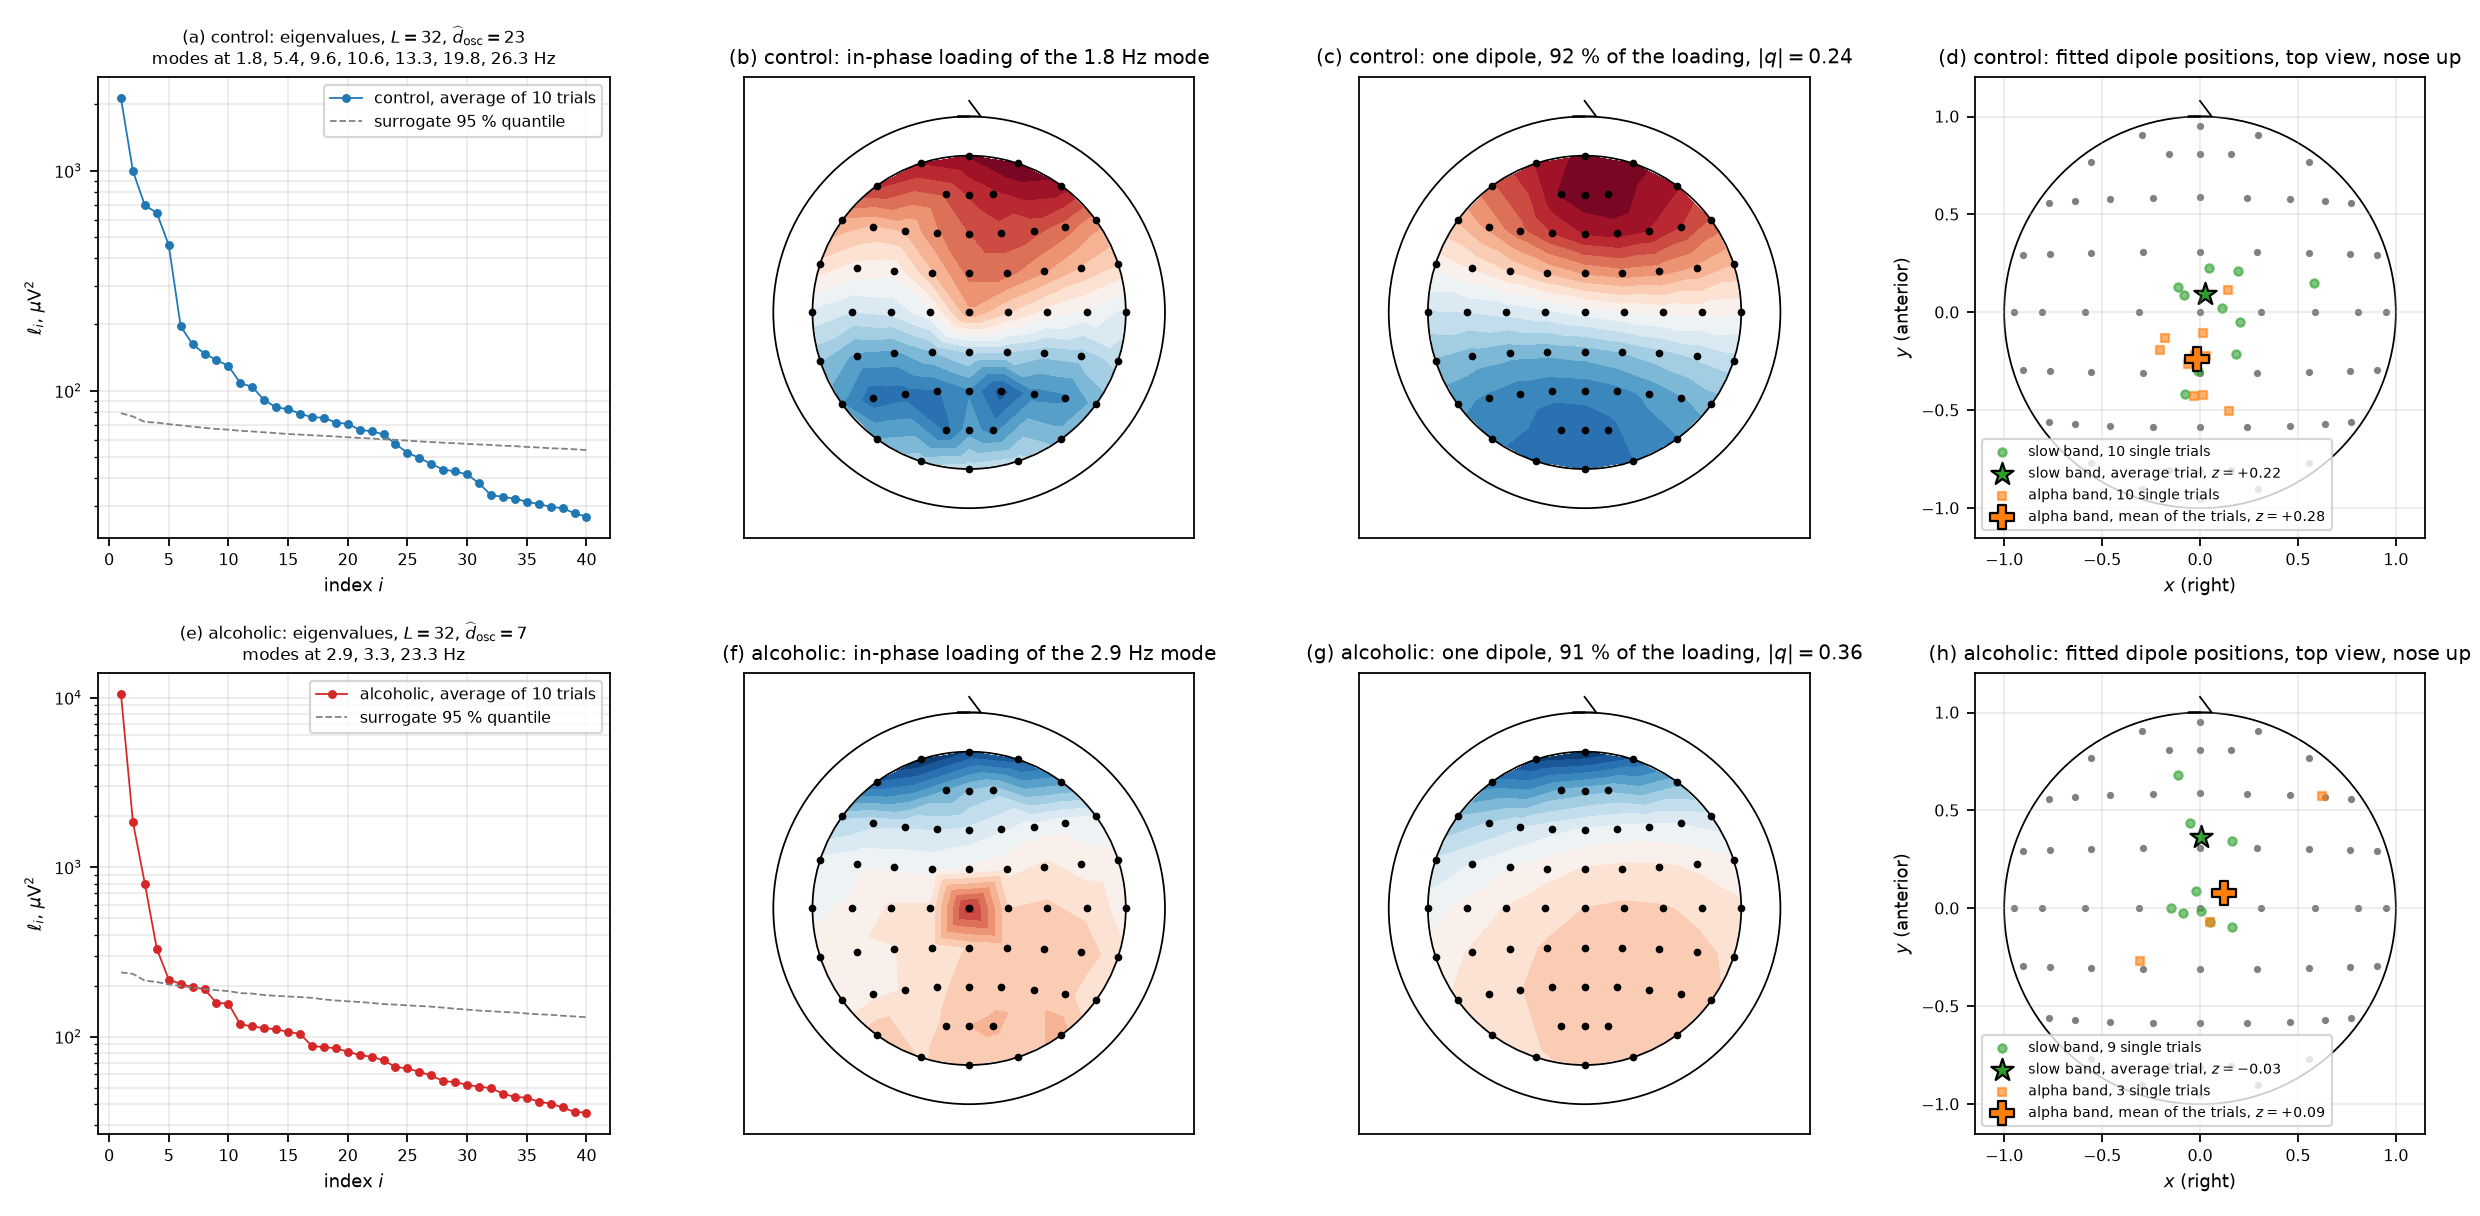
\includegraphics[width=0.99\textwidth]{fig8_real_localization.png}
    \caption{The algorithm of Section~\ref{sec:mssa-assisted-inverse-localization} on two subjects of the UCI EEG database \cite{ref-UCI}: gain matrix of a current dipole in a homogeneous sphere, $61$ electrodes at the ideal 10--10 positions, average reference, $L = 32$. Top row, the control subject; bottom row, the alcoholic subject. (a, e) Eigenvalues of the block-Hankel matrix of the average of the ten trials against the $95\,\%$ quantile of the surrogates, with the count and the frequencies of the modes read from the poles. (b, f) In-phase loading of the slow evoked wave ($1.8$ and $2.9$ Hz) as a scalp map: electrodes as dots, the outer circle the equator of the sphere, the inner one the ring of Fpz, T7, Oz and T8, nose up. (c, g) The loading predicted by one dipole fitted to it, with the explained fraction and the depth $|q|$ in units of the head radius. (d, h) Fitted dipole positions in the top view: slow band, a star for the average trial and circles for the single trials; alpha band, squares for the single trials and a cross for their mean; the $z$ coordinates in the legend. Generated by \texttt{fig\_real\_localization.py} from the archive \texttt{smni\_eeg\_data.tar.gz} of the UCI database \cite{ref-UCI}.}
    \label{fig:real}
\end{figure}

\begin{figure}[tb]
\renewcommand{\figurename}{Fig.}
    \centering
    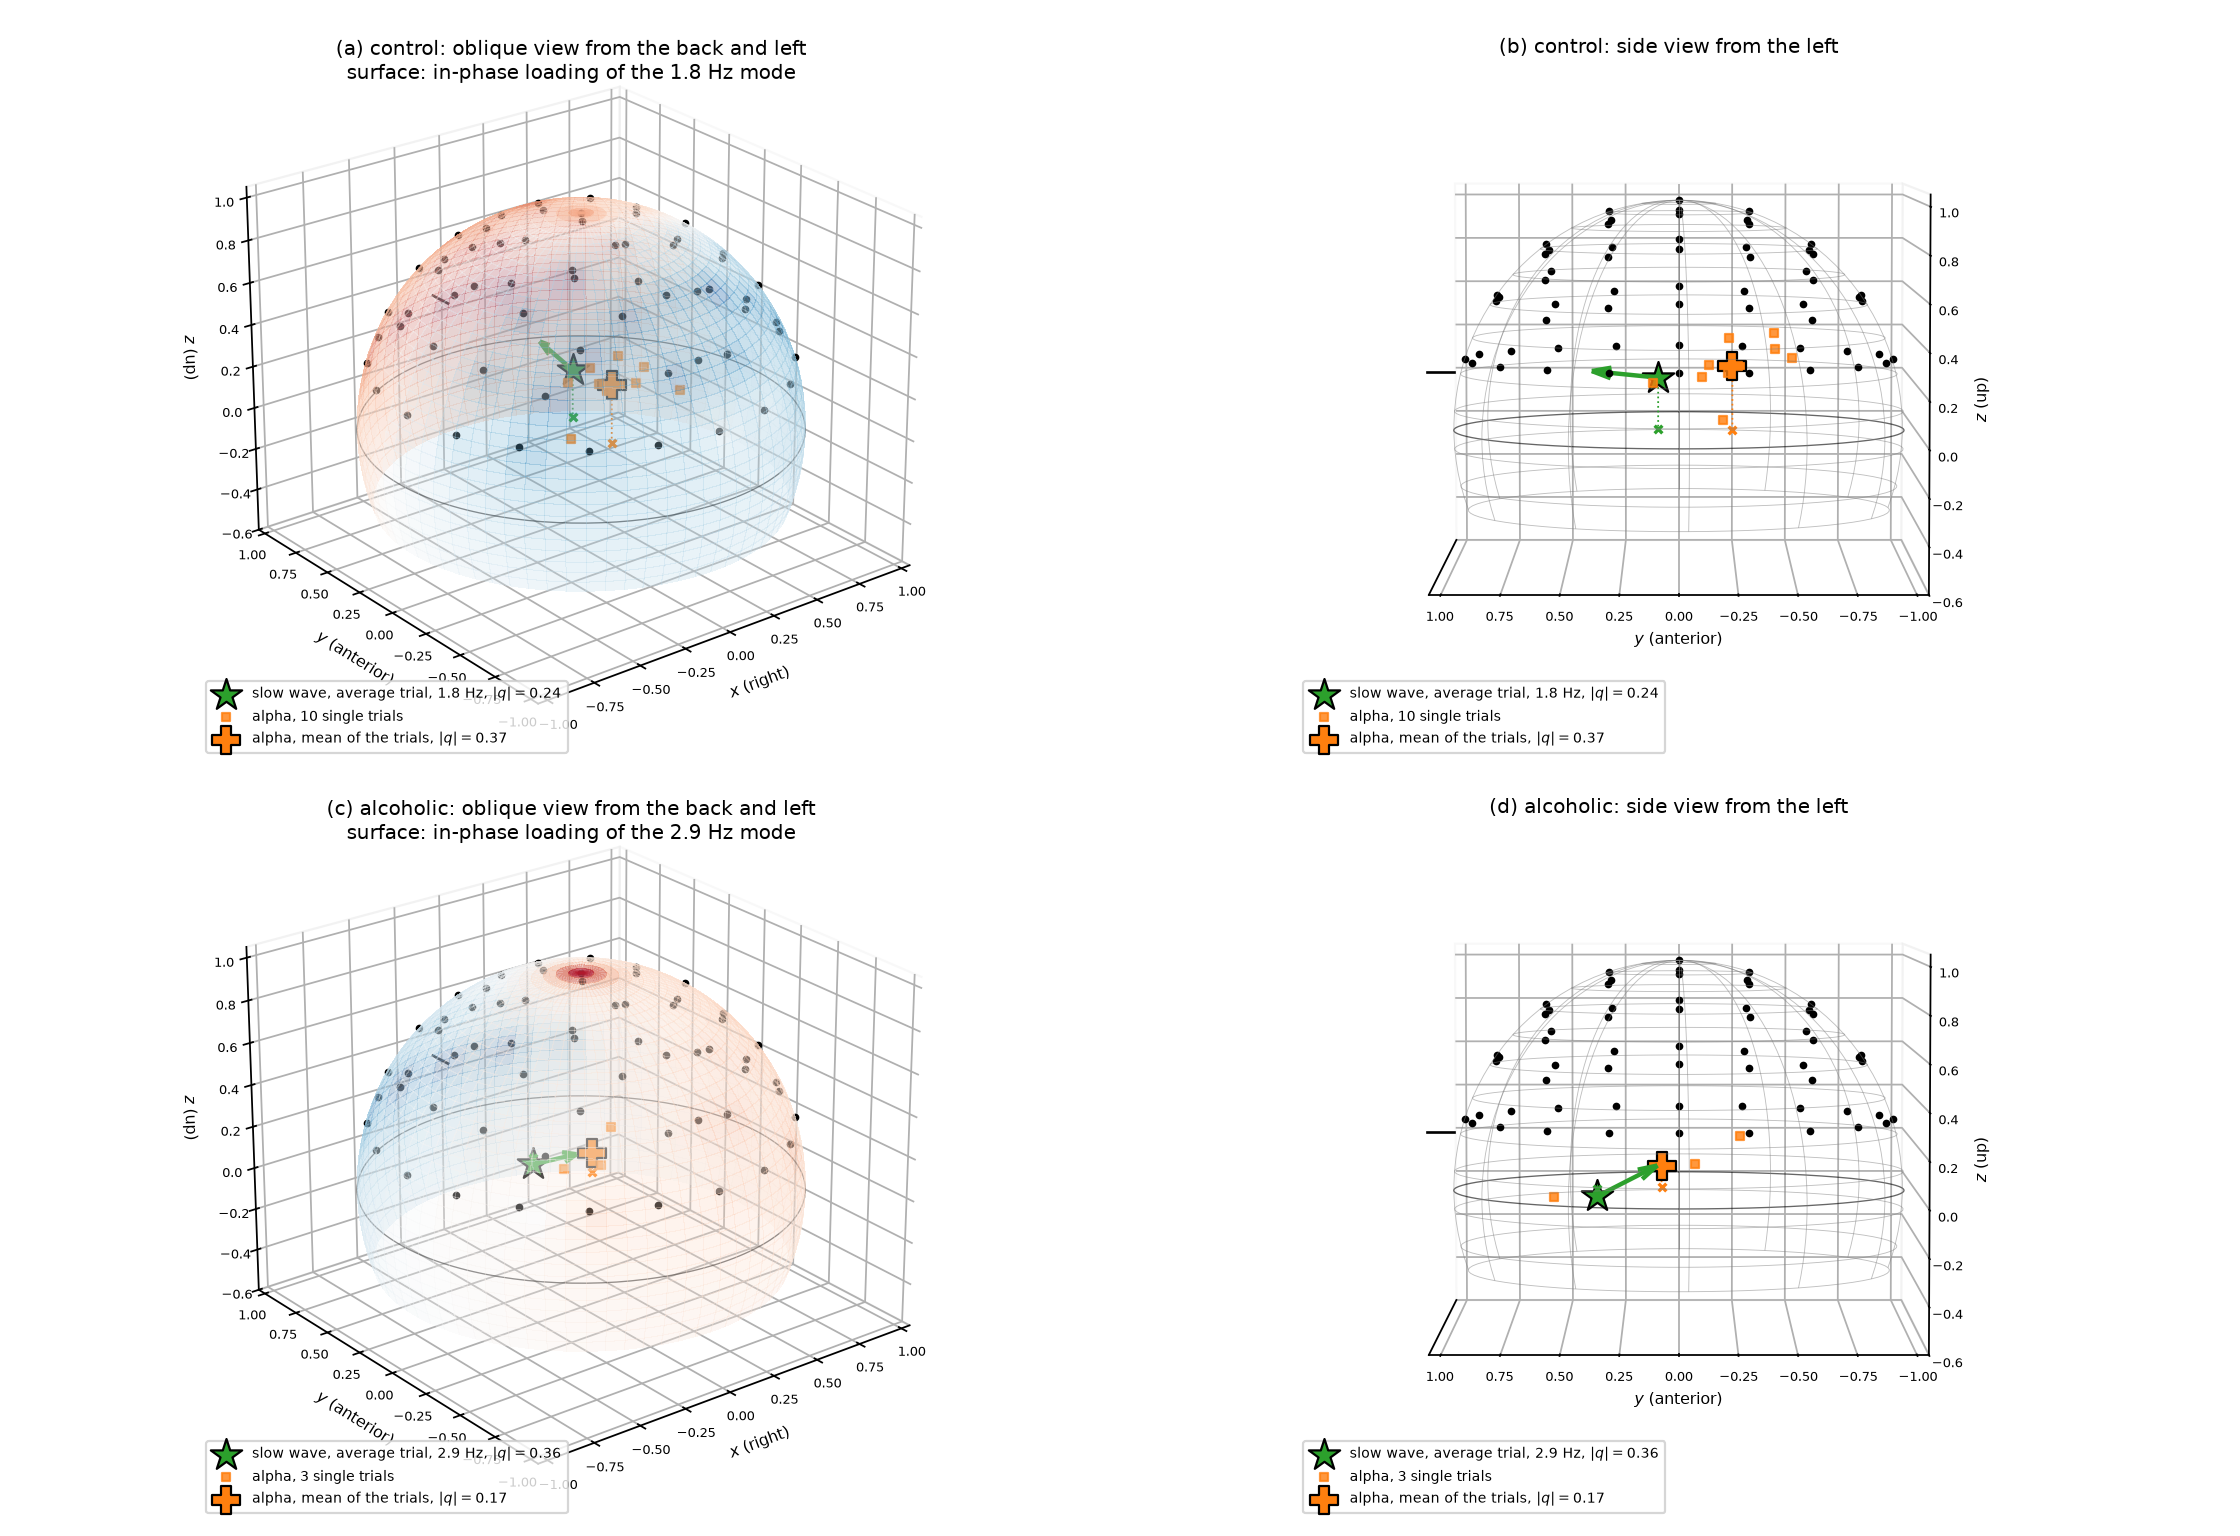
\includegraphics[width=0.99\textwidth]{fig9_real_3d.png}
    \caption{The sources of Fig.~\ref{fig:real} inside the head model: the unit sphere of the forward model with the $61$ electrodes, the equator drawn, the nose marked. (a, c) Oblique view from the back and left; the surface carries the in-phase loading of the slow evoked wave interpolated between the electrodes (red positive, blue negative), the star is the dipole fitted to it in the average trial with an arrow along its moment, the squares are the alpha-band dipoles of the single trials and the cross their mean; a dotted drop line from every source to the equatorial plane marks its depth. (b, d) Side view from the left of the same objects. Top row, the control subject: the alpha dipoles cluster in the parieto-occipital region above the equator, the slow-wave dipole sits near the centre. Bottom row, the alcoholic subject: the slow-wave dipole lies in the frontal half at the level of the equator, and the three alpha fits do not cluster. Generated by \texttt{fig\_real\_3d.py} from the fits written by \texttt{fig\_real\_localization.py}.}
    \label{fig:real3d}
\end{figure}

\section{Numerical experiments}\label{sec:numerical-experiments}

The positions of sources are not known in the recordings on which the count was developed \cite{ref-BernadotteBuchstaber, ref-Bernadotte05, ref-companionA}, so the experiments of this section are simulations; Section~\ref{sec:mssa-assisted-inverse-localization} shows the procedure on real EEG without ground truth.

\subsection{Setting}\label{sec:setting}

Unless stated otherwise, nine sensors form a $3 \times 3$ grid on the unit square ($d = 2$), so that lengths are in units of the side of the array. The sampling rate is 100 Hz, $N = 500$ (five seconds) and $L = 40$. Sources are undamped sinusoids of random phase at random positions in $[0.1, 0.9]^2$, at least 0.12 from every sensor. The attenuation law is $g(\rho) = \rho^{-1}$, or $e^{-3\rho}$ where indicated. Sensor noise is white, Gaussian and of equal variance $\sigma_\varepsilon^{2}$ in all channels. The signal-to-noise ratio is defined at the reference distance $\rho_0 = 0.5$, \[
\mathrm{SNR}_0 = \frac{\alpha^{2}\, g(\rho_0)^{2}}{2\, \sigma_\varepsilon^{2}},
\] the ratio that a source of amplitude $\alpha$ has at a sensor half an array side away. Position errors above 0.1 are called gross. Each point is the result of 300 trials unless noted. In Sections~\ref{sec:one-source}--\ref{sec:a-dipolar-source} the rank is given, so that the localization step is tested separately; in Section~\ref{sec:the-complete-procedure} it is estimated.

\subsection{The exact statements}\label{sec:the-exact-statements}

Without noise the statements of Sections~\ref{sec:second-inverse-problem-recovering}--\ref{sec:special-cases-of-attenuation} hold to machine precision; the rank and loading checks are in \cite{ref-companionA}.

\emph{Ambiguities} (Fig.~\ref{fig:ambiguity}). With eight sensors on a circle and a power law, the profiles of a point and of its inverse in the circle coincide to $10^{-16}$ for $\gamma = 0.5$, 1 and 2, and differ for the exponential law. With three sensors the twin is the inverse in the circumscribed circle. With sensors on a line it is the mirror image, for both laws. With the grid of nine sensors there is no twin. For the exponential law and three sensors in the plane a second exact solution exists for 6 of 200 source positions, and for none with four sensors of a random array; four sensors on one branch of a hyperbola are the exception (Proposition~\ref{prop:levels}): their profiles for the two foci agree to $4 \times 10^{-16}$ although no three of them are collinear. Of $20\,000$ five-sensor arrays drawn uniformly in the unit square, $1202$ ($6.0\,\%$) lie on one branch of a hyperbola and are ambiguous for the exponential law, while none of $2000$ six-sensor arrays lies on a conic. In $\mathbb{R}^{3}$, for seven sensors on a sheet of a hyperboloid of revolution, the $7 \times 7$ Jacobian of the system in $(q, q', \Delta)$ has smallest singular value between $4 \times 10^{-4}$ and $4 \times 10^{-3}$ against a largest of about $4$ in five random sheets, nonsingular in every case, and a perturbation of the sensors by $10^{-5}$ moves the ambiguous pair without destroying it. The Veronese matrix of Corollary~\ref{cor:quadric} has full rank $6$ for the grid of nine sensors and for six random sensors, rank $5$ for eight sensors on a circle, whose kernel is the circle, and rank $3$ for six sensors on a line. In three dimensions a point inside a sphere of twelve sensors and its inverse have the same profile to $10^{-16}$. The differential of the normalized map has a smallest singular value of $10^{-16}$ when the sensors lie on a circle or on a line through the source, and of order one otherwise (Theorem~\ref{thm:power-law}).

\emph{Shared mode.} For two sources at 10 Hz in quadrature, the plane spanned by the real and imaginary parts of the loading contains both fingerprints to $10^{-15}$ (Proposition~\ref{prop:shared-mode}), and the scan of Section~\ref{sec:two-sources-in-one} returns both positions to $10^{-10}$ in 100 of 100 configurations; on a $361 \times 361$ grid over the array the scan $\mathcal{J}$ falls below $10^{-6}$ at exactly two points, the two sources (Theorem~\ref{thm:plane-scan}). Matching the modulus of the loading to a single profile gives a position 0.12 away from either source (median).

\emph{Closed forms.} The linear systems of Section~\ref{sec:special-cases-of-attenuation} return the position to $10^{-13}$.

\begin{figure}[tb]
\renewcommand{\figurename}{Fig.}
    \centering
    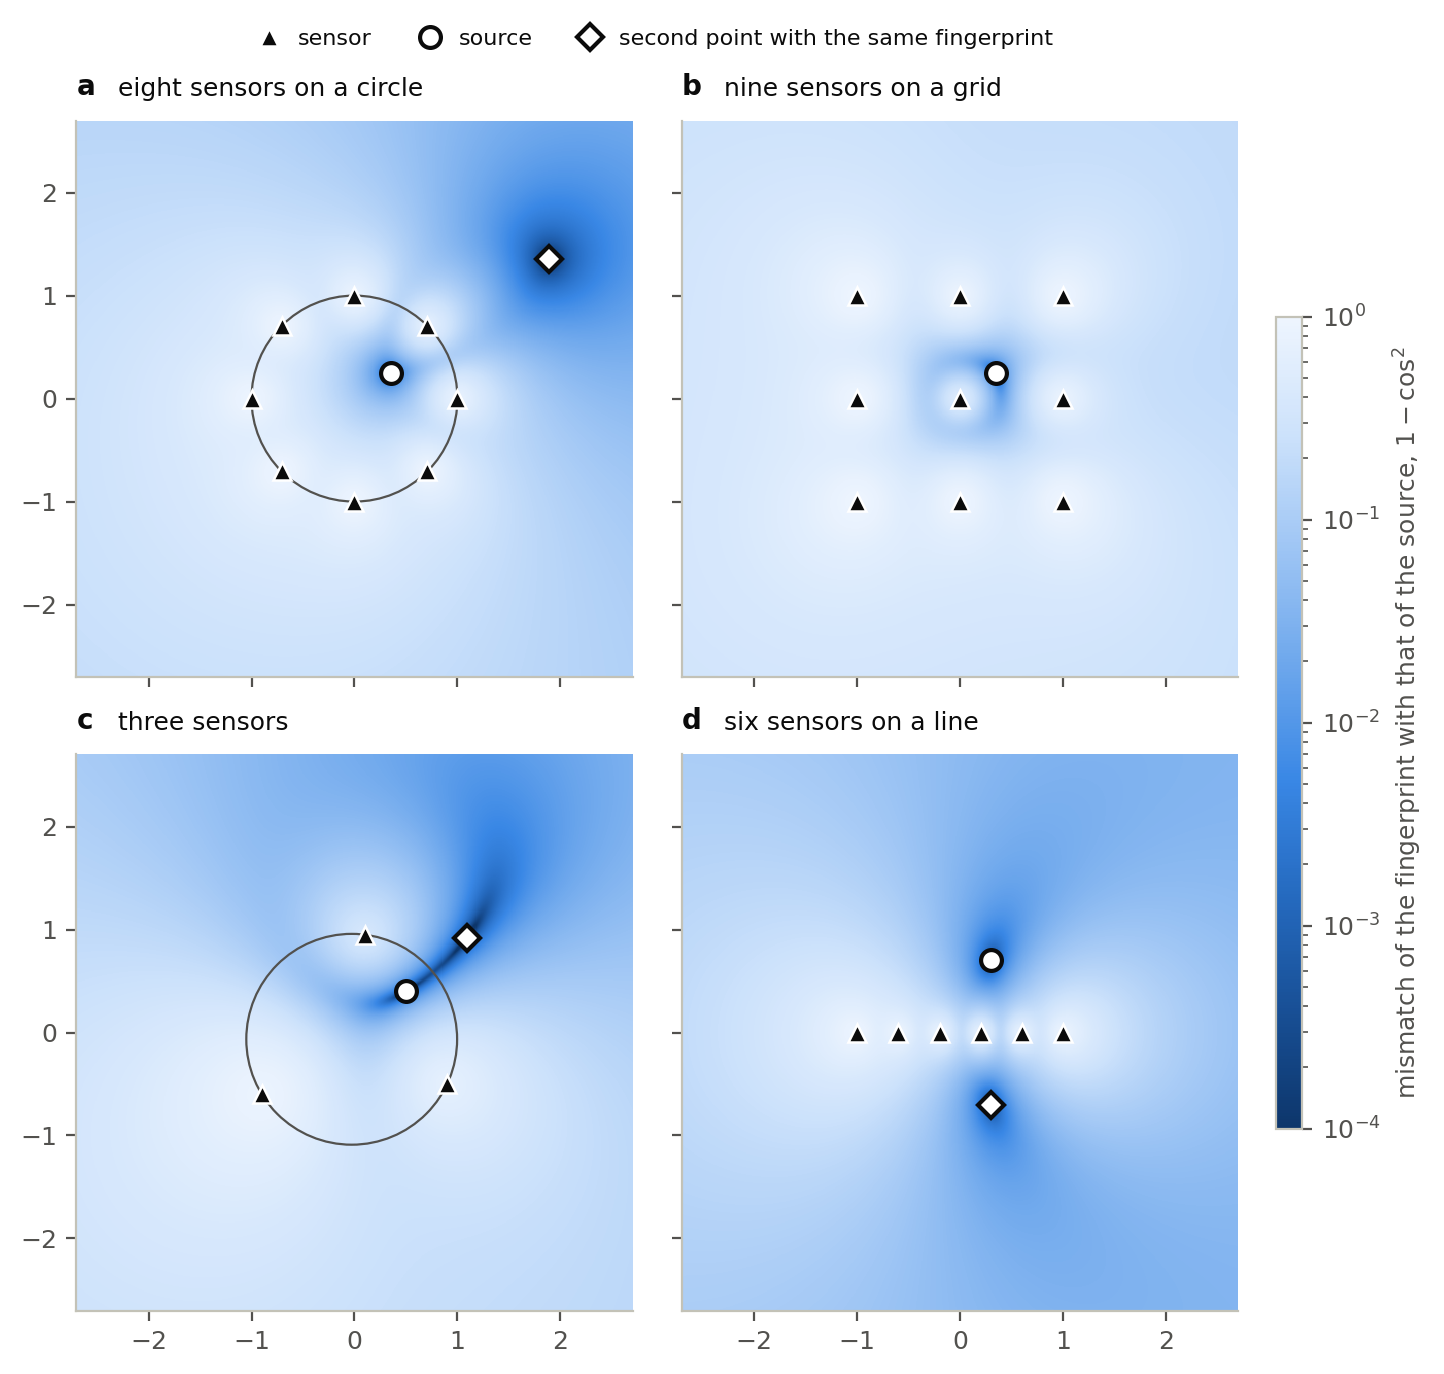
\includegraphics[width=0.82\textwidth]{fig1_ambiguity.png}
    \caption{Where the fingerprint is ambiguous: mismatch $1 - \cos^2$ between the attenuation profile of each point of the plane and that of the source, for power-law attenuation. (a) Sensors on a circle: the inverse of the source in the circle has the same normalized fingerprint. (b) Sensors on a grid: no second point. (c) Three sensors: the twin is the inverse in the circumscribed circle. (d) Sensors on a line: the mirror image.}
    \label{fig:ambiguity}
\end{figure}

\subsection{One source}\label{sec:one-source}

Table~\ref{tab:one-source} and Fig.~\ref{fig:accuracy}a, b give the position error for four ways of obtaining the fingerprint: the signed loading of Theorem~\ref{thm:loadings}, its modulus, the energy of the leading pair of singular vectors in every channel block, and the amplitude from the power in a band of $\pm 1$ Hz around the true frequency, which the other three do not know.

\begin{table}[htb]
\centering
\caption{One source, power law: RMS position error.}
\label{tab:one-source}
\begin{tabular}{l c c c c c}
\toprule
SNR$_0$ (dB) & signed loading & modulus & singular pair & band power & prediction \eqref{eq:accuracy} \\
\midrule
$-15$ & 0.084 & 0.083 & 0.084 & 0.107 & 0.067 \\
$-10$ & 0.041 & 0.042 & 0.044 & 0.050 & 0.038 \\
$0$ & 0.012 & 0.012 & 0.012 & 0.013 & 0.012 \\
$10$ & 0.0039 & 0.0039 & 0.0041 & 0.0040 & 0.0038 \\
$20$ & 0.0011 & 0.0011 & 0.0012 & 0.0012 & 0.0012 \\
\bottomrule
\end{tabular}
\end{table}

From $-10$ dB upward the error follows the first-order prediction within 10 \%, for both laws. Below $-15$ dB the mode is no longer found and every method fails. For a single source the choice of fingerprint is immaterial: the three MSSA variants agree within a few per cent, and band power at the known frequency is 5--30 \% worse up to 0 dB and within a few per cent above it. The decomposition, then, is not what makes one source more accurately located. Its contribution lies in separating several sources and in counting them.

\begin{figure}[tb]
\renewcommand{\figurename}{Fig.}
    \centering
    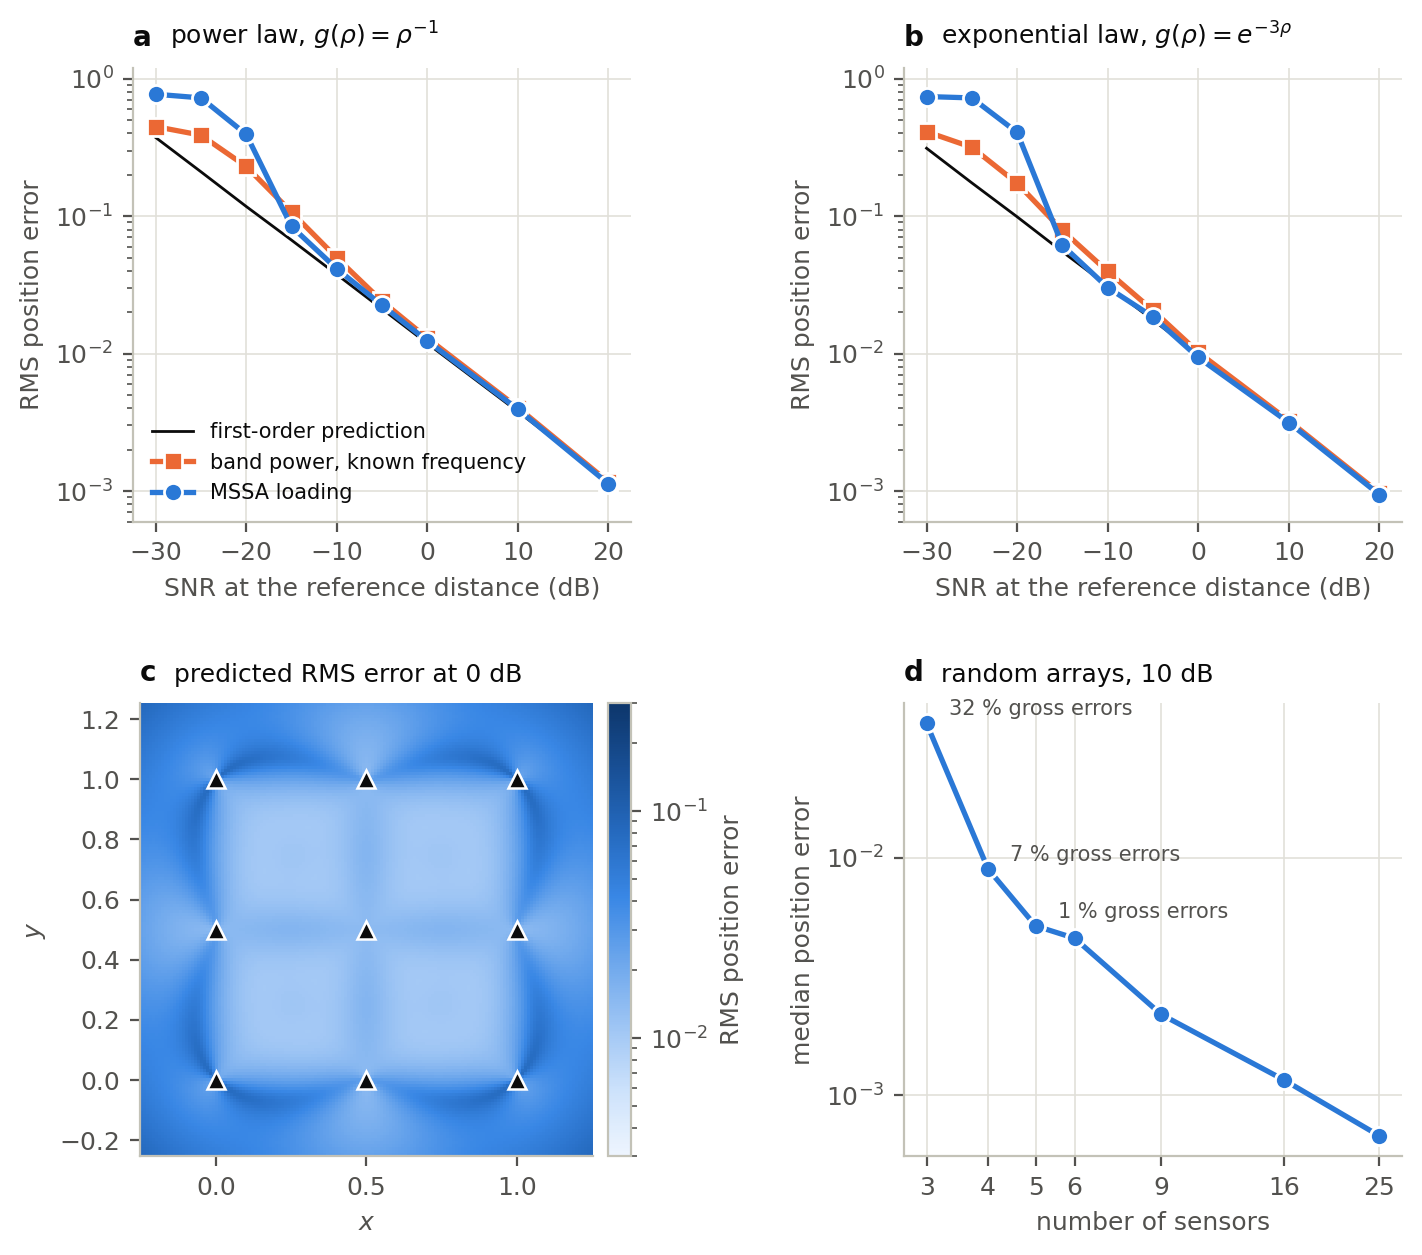
\includegraphics[width=0.88\textwidth]{fig2_accuracy.png}
    \caption{Accuracy for one source. (a, b) RMS position error against SNR for the MSSA loading and for band power at the known frequency, with the prediction of \eqref{eq:accuracy}, for the two attenuation laws. (c) Predicted RMS error over the plane at 0 dB for the grid of nine sensors (triangles); the error grows along circles that pass through neighbouring sensors, where the differential of the normalized map is close to singular (Theorem~\ref{thm:power-law}). (d) Median error against the number of sensors for random arrays at 10 dB, with the share of gross errors.}
    \label{fig:accuracy}
\end{figure}

\subsection{Two sources of different frequency}\label{sec:two-sources-of-different}

\emph{Strength.} Two sources at 10 and 13 Hz, at 10 dB, were localized from the loadings of Theorem~\ref{thm:loadings} and from pairs of singular vectors (Fig.~\ref{fig:two-sources}a). The former give a median error of 0.004--0.009 at every ratio of strengths, with no gross errors. The latter fail when the strengths are close: the median error is 0.34 with 97 \% gross errors at equal strength, 0.14 at a ratio of 1.05, 0.064 at 1.1 and 0.018 at 1.25, and the two methods coincide only from a ratio of 2. Singular vectors are a basis of the signal subspace, not a list of sources.

\emph{Frequency separation.} With equal strengths and a separation of half the Fourier resolution $1/T = 0.2$ Hz, both sources are localized with a median error of 0.008 at 10 dB and 0.003 at 20 dB, about twice the error at large separations (0.004 and 0.0013); at a quarter of the resolution the error is 0.025 and 0.008 (Fig.~\ref{fig:two-sources}b).

\emph{Position.} Two sources 3 Hz apart are localized equally well whether they are at one position or at different ones (0.0039 and 0.0041), and the same holds at a separation of one Fourier resolution. Closer than that, distinct fingerprints are what separates them: at a quarter of the resolution two sources at different positions are localized with a median error of 0.023, and two sources at one position are not separated at all (gross errors in 85 \% of trials).

\begin{figure}[tb]
\renewcommand{\figurename}{Fig.}
    \centering
    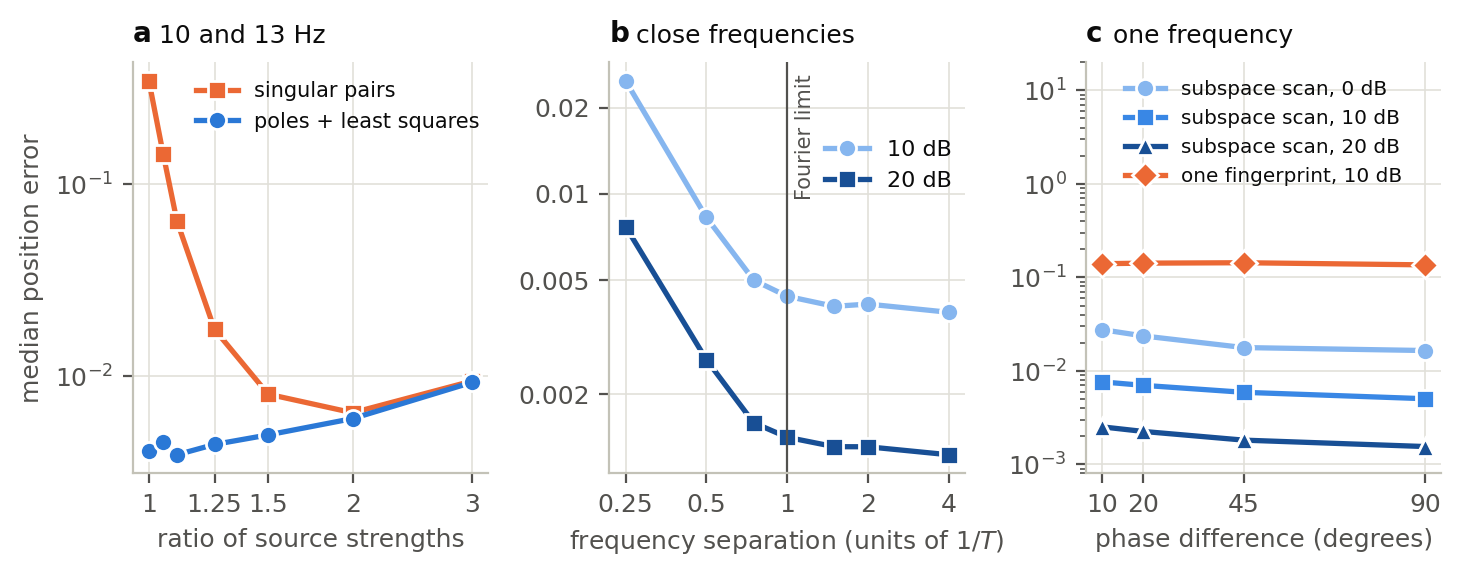
\includegraphics[width=1\textwidth]{fig3_two_sources.png}
    \caption{Two sources. (a) Different frequencies: median error of the worse-located source against the ratio of source strengths, for loadings from poles and least squares and for pairs of singular vectors. (b) Median error against the frequency separation in units of the Fourier resolution. (c) One frequency: subspace scan for two sources, and matching of a single fingerprint, against the phase difference.}
    \label{fig:two-sources}
\end{figure}

\subsection{Two sources of one frequency}\label{sec:two-sources-of-one}

For a single source the in-phase test at the 5 \% level rejects in 4.2, 4.3 and 5.5 \% of 1000 trials at 0, 10 and 20 dB, as it should. For two sources at 10 Hz it detects the second source in 83 \% of trials at a phase difference of 10$^{\circ}$ and 0 dB, in 98 \% at 20$^{\circ}$, and in all trials at larger phase differences or higher SNR. The subspace scan then localizes both sources with a median error of 0.016--0.028 at 0 dB, 0.005--0.008 at 10 dB and 0.0016--0.0025 at 20 dB, with gross errors in 1--3 \% of trials at 10 dB and above and in 2--13 \% at 0 dB (Fig.~\ref{fig:two-sources}c). Matching a single fingerprint to the same mode gives a position 0.14 away from the nearer source, whatever the SNR.

\subsection{Sensors and the attenuation law}\label{sec:sensors-and-the-attenuation}

\emph{Number of sensors.} For random arrays at 10 dB (Fig.~\ref{fig:accuracy}d; 20 arrays of each size, 30 sources each), three sensors give gross errors in 32 \% of trials: the second solution of Corollary~\ref{cor:sensors}(ii) lies inside $\Omega$ for part of the source positions. Four sensors give 7 \%, five 1 \%, and six or more none; four random sensors are never exactly on a circle but are often close to one. The median error falls from 0.009 with four sensors to 0.002 with nine and 0.0007 with twenty-five.

\emph{Attenuation exponent.} When the fit assumes an exponent different from the true $\gamma = 1$, the position is biased (Fig.~\ref{fig:models}a): at 0 dB the median error is 0.009 with the true exponent, 0.016--0.018 with an exponent wrong by 10 \%, 0.032--0.035 with one wrong by 20--25 \%, and 0.075--0.080 for exponents of 0.6 and 2. Estimating the exponent together with the position costs little: the median position error is 0.010, and the estimated exponent has a median of 1.00 and an interquartile range of 0.97--1.03.

\subsection{A dipolar source}\label{sec:a-dipolar-source}

A current dipole was placed in the upper half of a unit ball, at a distance of 0.3--0.7 from the centre, and its potential in a homogeneous conductor was recorded by 32 sensors on the upper hemisphere; the orientation was varied from radial to tangential (200 trials per point). The fit with the gain matrix of Section~\ref{sec:gain-matrix-models} localizes the dipole with a median error of 0.0006--0.0008 at 20 dB and 0.007 at 0 dB at every orientation (Fig.~\ref{fig:models}b). The distance-only law with $\gamma = 2$, fitted to the absolute loading, is in error by 0.21--0.26 of the radius at every orientation, including the radial one. A homogeneous conductor is the simplest volume conductor; a realistic head model changes the gain matrix and not the procedure.

\subsection{The complete procedure}\label{sec:the-complete-procedure}

\emph{Three sources with the rank estimated.} Three sources with frequencies between 5 and 30 Hz at least 2 Hz apart, amplitudes between 0.7 and 1.3 and mutual distances above 0.2 were processed by the algorithm of Section~\ref{sec:mssa-assisted-inverse-localization} with the calibrated threshold of \cite{ref-companionA} ($\kappa = 0.135$). The rank is correct in 97--98 \% of recordings from $-15$ dB to 20 dB, in 19 \% at $-20$ dB and never at $-25$ dB (Fig.~\ref{fig:models}c). When it is correct, the RMS position error equals the first-order prediction from $-5$ dB upward: 0.0215, 0.0128, 0.0039 and 0.0013 at $-5$, 0, 10 and 20 dB against 0.0221, 0.0124, 0.0040 and 0.0013 (Fig.~\ref{fig:models}d). At $-10$ dB it is 0.039 after exclusion of 2 \% gross errors, and at $-15$ dB a fifth of the positions are gross errors.

The thresholds for the number of components are compared on the same recordings in \cite{ref-companionA}: the calibrated threshold is correct in 96--99 \% of trials from $-15$ dB upward, and the surrogate threshold, which inherits the power of a strong source, misses a weak one at amplitude ratios of ten and above.

\begin{figure}[tb]
\renewcommand{\figurename}{Fig.}
    \centering
    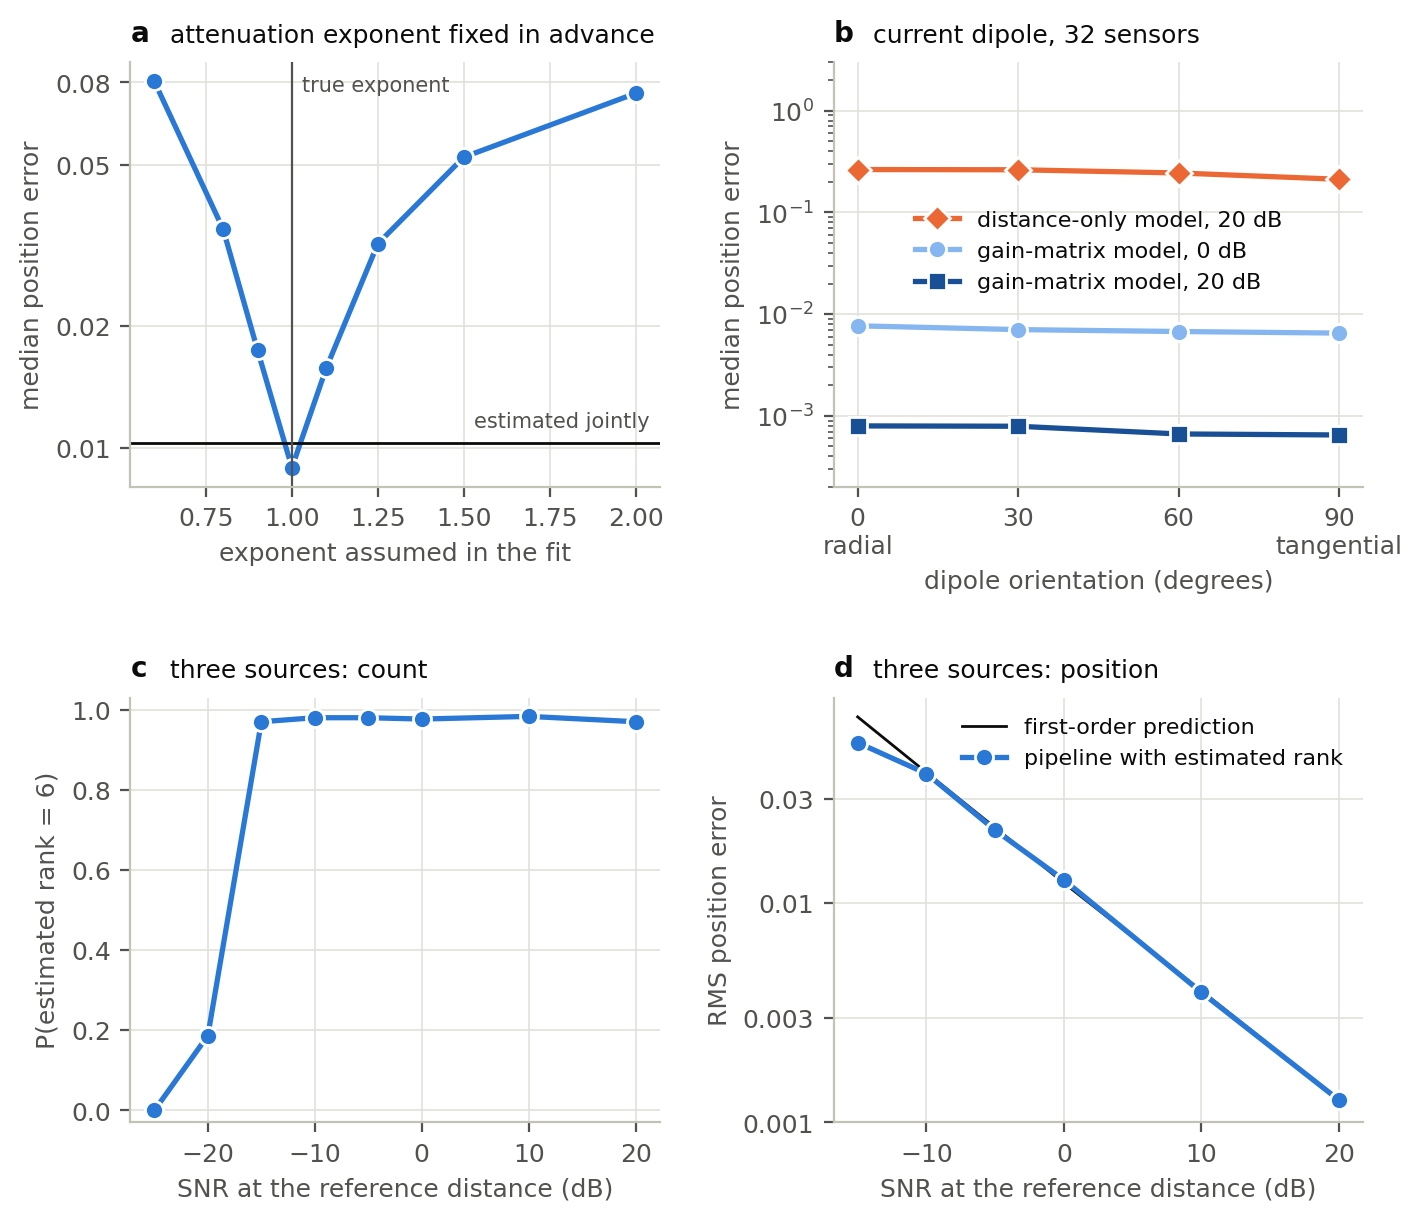
\includegraphics[width=0.88\textwidth]{fig4_models_pipeline.png}
    \caption{Models and the complete procedure. (a) Median position error when the attenuation exponent is fixed in advance at a value that may differ from the true one; the horizontal line is the error when the exponent is estimated together with the position. (b) Current dipole: gain-matrix model and distance-only model against the orientation of the dipole. (c) Three sources: probability that the estimated rank is correct. (d) Three sources: RMS position error of the procedure with estimated rank, and the prediction of \eqref{eq:accuracy}.}
    \label{fig:models}
\end{figure}

\subsection{Accuracy against the first-order prediction}\label{sec:guarantees}

The accuracy formula was checked end to end with the script \texttt{v2\_checks.py}. For one source on a $3 \times 3$ grid with $\gamma = 1$, the loading estimated by least squares at the known frequency and the position by Gauss--Newton matching, the measured root-mean-square error divided by the prediction $\frac{\sigma_\varepsilon}{\alpha}\sqrt{2/N}\,\mathcal{D}(q)$ is $1.00$, $1.04$, $1.01$, $0.98$, $0.99$ and $0.96$ for $N = 500$, $2000$, $8000$ at two noise levels (Proposition~\ref{prop:crb}). The checks of the count --- the noise floor against the Marchenko--Pastur edge, the signal eigenvalues against $\lVert a_k \rVert^{2} L/4$, and the exact count against the practical rule with $200$ trials per setting --- are reported in \cite{ref-companionA}.

\subsection{Robustness to model mismatch}\label{sec:robustness}

Version 1 \cite{ref-MSSAv1} tested two mismatches, an error in the exponent of the attenuation law and a coloured noise background. Three others are tested here with the complete procedure of Section~\ref{sec:the-complete-procedure} --- calibrated count, ESPRIT poles, least-squares loading at the estimated frequency, matching from a grid start --- for one source on the grid of nine sensors at $\mathrm{SNR}_0 = 10$ dB, $300$ trials per setting, errors in units of the array side (\texttt{v2\_robustness.py}). Without mismatch the count is $2$ in $94$--$97\,\%$ of trials from $0$ to $20$ dB, the $5\,\%$ of the calibration, and the position error is $0.011$, $0.007$, $0.004$ and $0.001$ at $0$, $5$, $10$ and $20$ dB with no gross error.

\emph{Errors in the sensor coordinates.} The coordinates used for matching are the true ones plus an isotropic Gaussian error of standard deviation $\sigma_p$. The position error grows from $0.004$ at $\sigma_p = 0$ to $0.007$, $0.011$, $0.022$ and $0.051$ at $\sigma_p = 0.005$, $0.01$, $0.02$ and $0.05$, with gross errors appearing at $0.05$ ($6\,\%$) and dominating at $0.1$ ($50\,\%$). The growth is linear and predicted to first order: an error $\delta p_j$ in a sensor enters the loading as an error $-g'(\rho_j)\, u_j^{\top} \delta p_j$ in its component, so with the notation of Proposition~\ref{prop:accuracy} the covariance of the position from sensor errors alone is $(J^{\top} \Pi_q^{\perp} J)^{-1} J^{\top} \Pi_q^{\perp}\, \mathrm{diag}\bigl(g'(\rho_j)^{2}\bigr)\, \Pi_q^{\perp} J\, (J^{\top} \Pi_q^{\perp} J)^{-1}\, \sigma_p^{2}$. Its root is $0.0054$, $0.011$, $0.022$ and $0.055$ at the four values of $\sigma_p$, and the measured error is the root of the sum of its square and the square of the noise term: $\sqrt{0.0037^{2} + 0.0054^{2}} = 0.0065$ against the measured $0.0067$ at $\sigma_p = 0.005$. For this array an error of $\sigma_p$ in every sensor coordinate costs about $1.1\,\sigma_p$ in the position.

\emph{Spatially correlated noise.} The sensor noise is white in time with covariance $\Sigma_{ij} = \exp(-\lVert p_i - p_j \rVert / l_c)$ across channels, of equal variance. The count with the calibrated threshold, which assumes an isotropic floor, is right in $98\,\%$ of trials at $l_c = 0$, in $75\,\%$ at $l_c = 0.25$ and in none at $l_c \ge 0.5$: the correlated part of the noise is a spatial component of its own, with an eigenvalue above the isotropic edge, and the rule counts too many modes. Whitening the recording with the noise covariance, $\widetilde{X} = \Sigma^{-1/2} X$, restores the count to $96$--$97\,\%$ at every $l_c$. Whitening changes the loadings as well, $\widetilde{a}_k = \Sigma^{-1/2} a_k$, and the experiment keeps track of this: the count and the poles are taken from $\widetilde{X}$; the loading is then estimated by least squares from the original recording at the estimated frequency, so that it stays in the sensor coordinates; and the matching whitens both the loading and the forward model, $\Sigma^{-1/2}\widehat{a}_k$ against $\Sigma^{-1/2} g_q$, which is generalized least squares with the known covariance and is equivalent to matching $\widehat{\widetilde{a}}_k$ to the transformed model and recovering $\widehat{a}_k = \Sigma^{1/2}\,\widehat{\widetilde{a}}_k$. The position is then unaffected: $0.004$ with or without whitening at every $l_c$, with no gross error. A spatially correlated background is therefore a problem of the first inverse problem, not of the second, and it is solved by the whitening that \cite{ref-companionA} prescribes for a coloured background in time; in practice $\Sigma$ is estimated from a segment without the sources, or from the residual after the modes are removed.

\emph{Propagation delays.} The source reaches sensor $j$ with a delay $\rho_j / v$, $v$ in array sides per second, which is absent from the instantaneous model \eqref{eq:model}. The rank stays $2$, since the delayed copies share the pole, and the complex loading of Theorem~\ref{thm:loadings} is $c_j = \alpha\, g(\rho_j)\, e^{-i\omega \rho_j / v}$: its modulus is the attenuation profile exactly and its phase carries the delay. Two consequences follow and are observed. First, the in-phase test of Proposition~\ref{prop:shared-mode} fails in every trial for every finite $v$ from $50$ downward, so a delayed single source is reported as two sources in one mode; delays and shared modes produce the same signature, and the model of Section~\ref{sec:sources-that-share-a} cannot tell them apart without a propagation model. Second, matching the modulus $|c_j|$ gives the position with the undelayed accuracy, $0.004$ and no gross error at every $v$, whereas matching the real part of the loading --- the fingerprint of an in-phase source --- fails once the phase spread is of order one: $0.027$ at $v = 50$, and gross errors in $75$--$99\,\%$ of trials at $v \le 20$. The procedure should therefore match the modulus of the complex loading whenever delays are possible; the phase is then additional information about the position, the time-difference-of-arrival measurement of hyperbolic positioning \cite{ref-Chan, ref-Torrieri}, which this paper does not use.

\subsection{Comparison with blind separation of independent components}\label{sec:comparison-with-blind-separation}

The count of \cite{ref-BernadotteBuchstaber, ref-Bernadotte05, ref-companionA} concerns temporal modes; sources within one mode, or within one band, have to be separated in space. Blind methods do this from the statistics of the mixture: independent component analysis from its non-Gaussianity \cite{ref-Comon, ref-Hyvarinen}, second-order blind identification (SOBI) from its lagged covariances \cite{ref-Belouchrani}. Each spatial pattern they return can then be matched to an attenuation profile by \eqref{eq:matching}, as dipoles are fitted to component maps in EEG \cite{ref-Delorme}. We compared this route with the procedure of Section~\ref{sec:mssa-assisted-inverse-localization} on two sources of equal strength at different positions, at 10 dB (Table~\ref{tab:blind}). The blind methods were applied to the recording band-passed around the sources and were given the number of components. For sources of one band the plane of Section~\ref{sec:two-sources-in-one} was taken from the two leading spatial singular vectors of the recording band-passed between 8 and 12 Hz.

\begin{table}[htb]
\centering
\caption{Two sources at different positions: median position error, with the share of gross errors in parentheses (10 dB; 200 trials for 5 s, 100 for 200 s). The bursts and the Gaussian signals are narrow-band signals at 10 Hz.}
\label{tab:blind}
\begin{tabular}{l c c c}
\toprule
source signals and record length & this procedure & FastICA, then \eqref{eq:matching} & SOBI, then \eqref{eq:matching} \\
\midrule
sinusoids at 10 and 13 Hz, 5 s & 0.004 (0 \%) & 0.005 (1 \%) & 0.005 (0 \%) \\
10 Hz sinusoids in quadrature, 5 s & 0.007 (1 \%) & 0.115 (56 \%) & 0.111 (57 \%) \\
10 Hz sinusoids 20$^{\circ}$ apart, 5 s & 0.027 (3 \%) & 0.18 (92 \%) & 0.19 (92 \%) \\
independent bursts, 5 s & 0.007 (1 \%) & 0.12 (59 \%) & 0.16 (65 \%) \\
independent bursts, 200 s & 0.0011 (2 \%) & 0.021 (1 \%) & 0.16 (72 \%) \\
independent Gaussian signals, 5 s & 0.007 (0 \%) & 0.12 (59 \%) & 0.13 (65 \%) \\
independent Gaussian signals, 200 s & 0.0011 (1 \%) & 0.12 (59 \%) & 0.14 (61 \%) \\
\bottomrule
\end{tabular}
\end{table}

When the sources differ in frequency, the three routes agree. When they share a frequency, the blind methods fail on records of five seconds, whatever the signals. For sinusoids the failure is one of principle. Two sinusoids in quadrature trace a circle; every rotation of the pair has the same distribution and the same lagged covariances, and neither criterion can choose among the rotations. Sinusoids 20$^{\circ}$ apart have a correlation of 0.94, which contradicts independence. The scan localizes both pairs, because the forward model, and not a statistical criterion, selects the two directions within the plane.

For independent sources the blind methods are limited by the record: in five seconds two narrow-band signals of one band have a sample correlation of 0.15--0.4. With longer records independent component analysis improves for the non-Gaussian bursts, with gross errors in 45 \% of trials at 20 s, 19 \% at 60 s and 1 \% at 200 s, where its median error is still twenty times that of the scan (Fig.~\ref{fig:blind}). It does not improve for Gaussian sources, which it cannot separate in principle \cite{ref-Comon}. SOBI needs sources with different spectra \cite{ref-Belouchrani} and fails at every length. Blind separation also returns no more sources than there are sensors: of twelve sinusoids of different frequencies recorded by nine sensors, the modes of Section~\ref{sec:mssa-spatial-loading-as} locate all twelve within 0.05, and independent component analysis with nine components locates 39 \%.

Two remarks delimit the result. First, for sources that are not sinusoids the temporal decomposition contributes little to the spatial step. The trajectory matrix then has many modes in the band (a median rank of 19 for the bursts and of 10 for the Gaussian signals), and the plane obtained from their loadings gives larger errors than the plane of the band-passed recording, 0.015 and 0.011 against 0.007. Second, the blind methods keep two uses that the scan does not have. They need no forward model, and for independent non-Gaussian sources on long records they return the waveforms of sources that share a band (correlation 0.99 with the true waveforms at 200 s), which the temporal modes do not separate.

\begin{figure}[tb]
\renewcommand{\figurename}{Fig.}
    \centering
    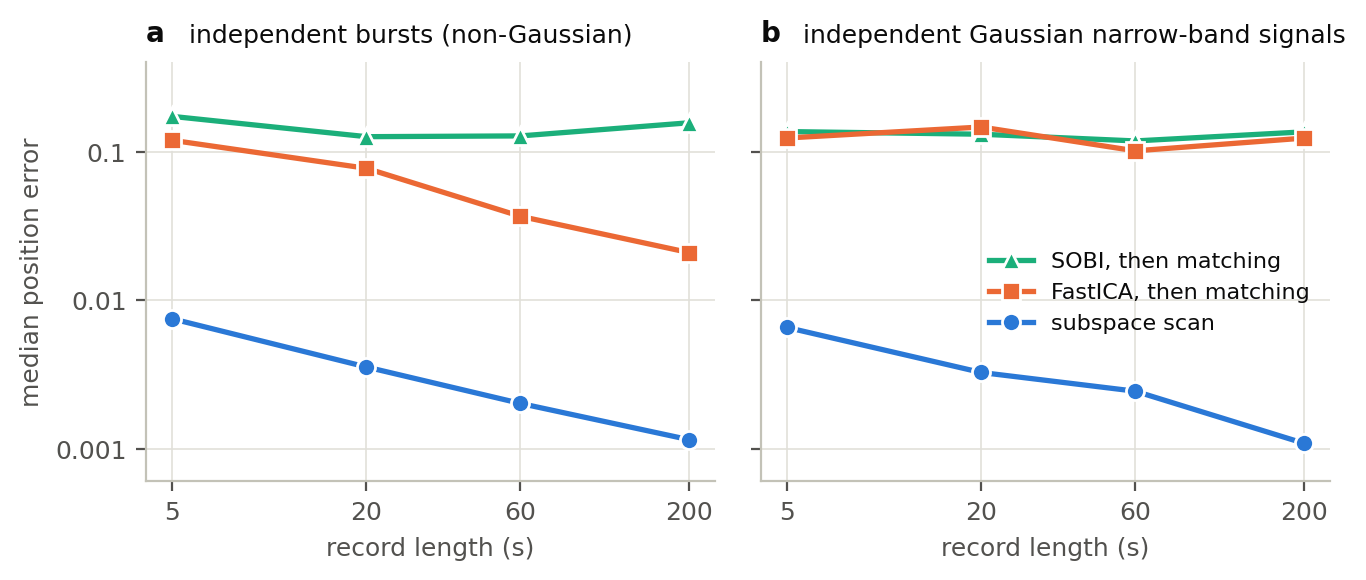
\includegraphics[width=0.88\textwidth]{fig5_blind_separation.png}
    \caption{Blind separation against record length: median position error for two independent sources of one band, located by the subspace scan and by blind separation followed by matching (10 dB). (a) Non-Gaussian bursts. (b) Gaussian narrow-band signals.}
    \label{fig:blind}
\end{figure}

\section{Applications}\label{sec:applications}

The method is general. It applies whenever multichannel observations are mixtures of latent oscillatory or quasi-oscillatory sources whose amplitudes attenuate across sensors, channels, features, or network positions. Like the source-number method of \cite{ref-BernadotteBuchstaber}, it is not tied to the brain, although EEG is where the framework was developed \cite{ref-BernadotteBuchstaber, ref-Bernadotte05, ref-Bernadotte10, ref-Bernadotte07, ref-Bernadotte06}.

\subsection{Neurophysiology and EEG/MEG}\label{sec:neurophysiology-and-eeg-meg}

In EEG/MEG, latent neural populations generate oscillatory activity recorded by multiple sensors. The attenuation profile is determined by distance, tissue conductivity, orientation, and lead-field geometry. It is therefore described by the gain-matrix model of Section~\ref{sec:forward-models-with-a} with the lead field of the head model, and not by a function of distance alone (Section~\ref{sec:a-dipolar-source}). MSSA can first estimate the number of active oscillatory modes \cite{ref-BernadotteBuchstaber, ref-Bernadotte05, ref-companionA} and then provide spatial loading patterns for inverse source localization; the fit of Section~\ref{sec:gain-matrix-models} is the counterpart, for oscillatory modes, of fitting dipoles to the maps of independent components \cite{ref-Delorme}.

Potential uses include localization of alpha, beta, theta, or gamma generators; detection of pathological oscillatory sources; sleep-stage and coma-state analysis \cite{ref-Bernadotte07}; BCI calibration; and neurofeedback personalization.

The count and the loadings also serve closed-loop protocols, among them the intelligent-feedback stimulation of chosen brain regions for rehabilitation and the prevention of neurodegeneration \cite{pat-feedback} and the activation of a preserved brain pattern \cite{pat-pattern}, both of which need a readout of the state of a region and a loading to address it. In neurofeedback and non-invasive stimulation for attention-deficit disorder \cite{ref-ADHD} the feedback variable is a band power; MSSA replaces it by the energy and the loading of an identified mode, so that the loop follows one oscillatory mode rather than a band that several sources share; the mode is a single physical source only when its loading passes the in-phase test of Proposition~\ref{prop:shared-mode} and the identifiability conditions of Section~\ref{sec:identifiability} hold. Downstream of the count, the modes and their loadings are the features of the brain--computer-interface pipeline: silent-speech recognition from EEG with convolutional and recurrent networks \cite{ref-Sensors}, the choice of a command dictionary by a statistical proximity criterion \cite{ref-CRMdict} and the algorithm that maximizes the accuracy of $k$-classification over representatives of $k$ classes \cite{ref-MathK, ref-DMA}, the quality criterion for clustering a tagged sample \cite{ref-ISCluster}, and the detection of frequency, time and spatial changes of the EEG after COVID-19 \cite{ref-CRMcovid, ref-ISCovid}; in each of these the number of oscillatory sources decides how many features are real, and the count itself, with its guarantees, is the subject of \cite{ref-companionA}.

\subsection{Robotic endovascular surgery}\label{sec:robotic-endovascular}

In the LevshAI robotic ecosystem for endovascular neurosurgery, a motion-copying manipulator with haptic feedback and a preoperative personalized vascular simulator \cite{ref-LevshAI-CBS, ref-LevshAI-sim}, the force and position channels of the instrument carry the cardiac and respiratory oscillations of the vessel wall and of the patient. Their number and their origin along the instrument are what the first inverse problem returns, before the oscillations are compensated in the haptic loop. The simulator supplies the geometry of the vessel tree for the forward model, segmented from angiography by lightweight networks \cite{ref-VeNet} trained on annotated data \cite{ref-SciData}. The remote link of such a system fixes what may be computed off-site \cite{ref-Cyber}; the MSSA stage is light enough to run on the manipulator side.

\subsection{Wearable sensor networks}\label{sec:wearable-sensor-networks}

In wearable systems, physiological or mechanical oscillations may be recorded by distributed sensors. Examples include cardiac and respiratory oscillations, tremor, gait oscillations, muscle activation patterns, and biomechanical vibrations. If signal amplitude decays with distance or sensor coupling, MSSA-derived spatial loadings can identify the location of the latent oscillatory source on the body or device network. A lightweight real-time implementation of the Hankel embedding exists \cite{ref-Bernadotte06}.

\subsection{Industrial monitoring and predictive maintenance}\label{sec:industrial-monitoring-and-predictive}

Rotating machines, turbines, engines, and mechanical structures often generate oscillations that propagate through a sensor network with attenuation. MSSA can separate latent vibration modes, estimate their number \cite{ref-BernadotteBuchstaber}, and localize their origin. Applications include fault localization, bearing defect detection, turbine vibration analysis, structural health monitoring, and acoustic emission localization.

The changes of the count over time form a symbolic stream of events. Matching patterns in that stream in real time, without the state explosion of classical automata, is the problem solved by counter-augmented deterministic automata \cite{ref-Automata, ref-Regex}, built on the structural automaton designs that avoid the exponential blowup of one class of regular languages \cite{ref-BernadotteAutomata, ref-ISStruct} and on automaton compression \cite{ref-ISCompress}; they make the MSSA stage a front-end for event detection in monitoring systems.

\subsection{Seismology and geophysics}\label{sec:seismology-and-geophysics}

Seismic or geophysical events generate waves recorded by spatially distributed sensors. When amplitude attenuation is known or calibrated, MSSA can separate oscillatory components, count them as in \cite{ref-BernadotteBuchstaber}, and use spatial loading profiles for source localization. Possible uses include microseismic event localization, volcanic tremor analysis, underground structural monitoring, and oceanographic oscillation source detection. Surface arrays are planar, the case of Corollary~\ref{cor:sensors}(iv).

\subsection{Wireless and electromagnetic systems}\label{sec:wireless-and-electromagnetic-systems}

In wireless sensor networks, oscillatory signals may be emitted by latent sources and recorded with power decay across receivers; their number is estimated as in \cite{ref-BernadotteBuchstaber}. The MSSA attenuation-fingerprint framework can support emitter localization, interference source detection, spectrum monitoring, and distributed antenna diagnostics.

\subsection{Financial sector}\label{sec:financial-sector}

The financial sector is not spatial, and we include it as the case that shows where the method stops. The first inverse problem and the loadings apply to any multichannel series. The second applies only if coordinates can be given to the channels independently of the data and an exposure-decay law can be verified; otherwise a recovered coordinate has no economic interpretation, and we make no claim that one exists.

Financial markets produce multichannel time series where channels may be asset returns, sector indices, volatility curves, yield-curve points, liquidity indicators, order-book features, macroeconomic indicators, or cross-market spreads. Latent oscillatory sources may represent business-cycle components, liquidity cycles, volatility regimes, sector rotation waves, risk-on/risk-off oscillations, intraday microstructure cycles, or hidden market stress modes.

Factor analysis of economic data has been formulated as an extremal problem on Grassmann manifolds \cite{ref-BuchstaberMaslov}, the geometry that underlies the unfolding of time series \cite{ref-Buchstaber}. The analogue of physical attenuation is factor-exposure decay across a feature space. A latent financial oscillator may affect some assets strongly and others weakly depending on their distance from the source in a financial similarity space. For example, coordinates $p_j$ may be assigned to assets or indicators in a latent embedding space constructed from sector membership, correlation distance, factor loadings, duration, maturity, liquidity, geography, market capitalization, or volatility-regime similarity.

A latent financial source at coordinate $q_k$ produces an oscillatory component with exposure \[
a_{jk} = \alpha_k\, g(d(p_j, q_k)),
\] where $d(p_j, q_k)$ is a financial distance and $g$ is an exposure-decay function. MSSA extracts latent oscillatory market modes $s_k(t)$ and their loadings $\widehat{a}_k$ across assets. The loading vector becomes an amplitude fingerprint of the latent financial source. Matching this fingerprint to candidate points in the financial feature space, by \eqref{eq:matching} with the profiles $g_q = (g(d(p_1, q)), \dots, g(d(p_m, q)))^{\top}$, can localize the source of the regime.

Two of the conditions of Section~\ref{sec:conditions-required-for-coordinate} need attention in this setting. The coordinates $p_j$ must be known independently of the loadings that are to be explained: an embedding constructed from the correlations of the same series is not independent of them, and matching against it is circular. Coordinates that exist beforehand satisfy the condition directly --- maturity along a yield curve, strike and maturity on a volatility surface, the geographical position of regional indices. And the exposure-decay function is not given by physics. It has to be chosen as a parametric family whose parameters are estimated together with the position, as the exponent is in Section~\ref{sec:sensors-and-the-attenuation}, and the residual fraction of Section~\ref{sec:one-source-per-mode} shows whether the family fits. On a yield curve, for example, the channels are yields at maturities $p_1 < \dots < p_m$, $d = 1$, and an oscillatory component with exposure $\alpha\, g(|p_j - q|)$ is located at a maturity $q$; three or more maturities determine $q$ uniquely for a power law (Theorem~\ref{thm:power-law} with $d = 1$).

Uses of this kind --- the maturity at which a cycle of the yield curve is centred, the position of a regime on a volatility surface --- are possibilities whose premises have to be verified case by case, not results of this paper; the count of latent oscillatory modes and their loadings are available in any case, a coordinate only under the two conditions above.

\section{Discussion}\label{sec:discussion}

This article, with its companion \cite{ref-companionA}, formulates MSSA as a method for two linked inverse problems in multichannel oscillatory systems. The first inverse problem is the recovery of the number of latent oscillatory sources, addressed in Bernadotte's Hankel-embedding framework \cite{ref-BernadotteBuchstaber, ref-Bernadotte05} and given its multichannel form and its guarantees in \cite{ref-companionA}.

The second inverse problem is the recovery of source coordinates. This becomes possible when each latent oscillatory source is observed with distance-dependent amplitude attenuation. In that case, the spatial loading vector recovered by MSSA is not merely a statistical component. It is an empirical amplitude fingerprint of the source location.

The coordinate recovery problem then reduces to matching this empirical fingerprint to a theoretical attenuation profile generated by candidate coordinates. The solution is unique when the normalized attenuation map is injective, the sensor geometry is non-degenerate, sources are temporally separable, spatial fingerprints are distinguishable where that is needed, and noise is sufficiently small. Sections~\ref{sec:identifiability} and \ref{sec:conditions-required-for-coordinate} turn each of these conditions into a statement that can be checked for a given array, law and recording.

This framework separates the inverse problem into two stages: \[
X \xrightarrow{\ \mathrm{MSSA}\ } (\widehat{r}, \widehat{a}_k, \widehat{s}_k) \xrightarrow{\ \text{attenuation matching}\ } \widehat{q}_k .
\] The first stage is structural. It identifies how many oscillatory sources are present and extracts their temporal modes and spatial loadings. The second stage is geometric. It maps spatial loadings to source coordinates using an attenuation model.

This separation is useful because the full inverse problem is typically ill-conditioned. MSSA regularizes it by reducing the raw multichannel signal to a finite set of coherent oscillatory components before spatial localization is attempted. The experiments locate the benefit. For one source the reduction changes little, and any amplitude fingerprint attains the accuracy that the geometry permits. With several sources it is what makes the problem separable: each source is fitted alone, in $d$ unknowns, whatever the strengths of the others, and their number is decided beforehand.

The central methodological claim is:

\begin{quote}
Multichannel Singular Spectrum Analysis converts a multichannel time series into a finite set of latent oscillatory modes. When the sources of these modes undergo amplitude attenuation across sensors, the MSSA spatial loading vector becomes an amplitude fingerprint of the source coordinate. Under known attenuation law, known sensor geometry, and injective source-to-sensor mapping, source coordinates are identifiable from these fingerprints.
\end{quote}

In formula form, $X \xrightarrow{\ \mathrm{MSSA}\ } \widehat{a}_k \approx \alpha_k\, g_{q_k}$, and therefore $\widehat{q}_k$ is given by \eqref{eq:matching}. This is the bridge between MSSA, source-number estimation, and coordinate recovery for attenuating oscillatory systems.

The count $\widehat{d}_{\mathrm{osc}}$ on which the procedure starts gives the Bernadotte Oscillator Intrinsic Dimension (BOID), introduced in \cite{ref-Bernadotte07} as the brain oscillator intrinsic dimension; its guarantees, and the distinction between the Hankel dimension, the number of modes and the number of generators, are in \cite{ref-companionA}. The present paper is about what the loadings of those modes say about where the generators are.

The scope of the present results is as follows. All experiments are simulations with white sensor noise that is independent between channels and of equal variance; a coloured or spatially correlated background, as in EEG, requires whitening before the count and reduces the gain from pooling channels. The forward model is instantaneous: propagation delays would add a phase to the loadings, which carries further information about position and is not used here. The attenuation law must be known up to a few parameters. Sources of one frequency and damping are resolved only two at a time, and not at all when they are in phase. The identifiability statements come in three strengths, local, generic and configuration-specific, with different sensor counts, and a claim about a given array is only the third (Proposition~\ref{prop:levels}); the efficiency of the position estimate is a statement about the loading observation model, not about the complete pipeline (Proposition~\ref{prop:crb}); and the count on which everything starts has its own conditions, stated in \cite{ref-companionA}. Blind separation of independent components remains the tool when no forward model is available, or when the waveforms of sources that share a band are wanted (Section~\ref{sec:comparison-with-blind-separation}). Validation on recordings with known source positions is the next step.

The method is not limited to EEG or BCI. It applies wherever latent oscillatory sources are observed through several channels with an attenuation that is a known function of a known geometry: sensor arrays in neurophysiology, wearable sensing, industrial monitoring, geophysics and wireless systems. Where the geometry is abstract and the attenuation law is not given by physics, as in the financial example of Section~\ref{sec:financial-sector}, only the first inverse problem and the loadings carry over without further assumptions; a recovered coordinate has a meaning only when the coordinates of the channels exist independently of the data and the exposure-decay law can be verified.


\section*{Code and data availability}\label{code-and-data-availability}
The identifiability checks of Section~\ref{sec:the-exact-statements} are reproduced by \texttt{v2\_identifiability\_checks.py}, the accuracy check of Section~\ref{sec:guarantees} by \texttt{v2\_checks.py}, the robustness experiments of Section~\ref{sec:robustness} by \texttt{v2\_robustness.py}, Fig.~\ref{fig:real} by \texttt{fig\_real\_localization.py} and Fig.~\ref{fig:real3d} by \texttt{fig\_real\_3d.py} from the fits the former writes; all are included with the source of this paper, together with their outputs, need only NumPy and Matplotlib, and are kept, with the experiments of version 1 \cite{ref-MSSAv1} and the \texttt{aicumene\_mssa} package, in the repository \url{https://github.com/aicumene/MSSA}. The embedding, the decomposition and the rank estimate use the \texttt{aicumene-mssa} package of that repository; pole estimation, loading extraction, the tests and the matching are in \texttt{paper/experiments/loc\_common.py} of the same repository, together with the scripts and numerical results of Section~\ref{sec:numerical-experiments}. The EEG trials of Fig.~\ref{fig:real} are from the public UCI EEG database \cite{ref-UCI}; the script reads them from the archive \texttt{smni\_eeg\_data.tar.gz} of that database. No other experimental data were used.

\renewcommand{\refname}{REFERENCES}
 \begin{thebibliography}{0}
\bibitem{ref-MSSAv1} Bernadotte A., Menshikov I. ``Multichannel Singular Spectrum Analysis for Estimating Oscillatory Sources and Localizing Attenuating Oscillations.'' Aicumene Preprint 2026.044v1. August 12, 2026. \href{https://doi.org/10.13140/RG.2.2.26719.01442}{doi:10.13140/RG.2.2.26719.01442}. \url{https://research.aicumene.com/papers/MSSA/}
\bibitem{ref-companionA} Bernadotte A., Menshikov I. ``Multichannel Singular Spectrum Analysis: Counting Oscillatory Modes and Recovering Their Spatial Loadings.'' Aicumene Preprint 2026.044v2; SSRN working paper 7693202 (November 11, 2026). \url{https://ssrn.com/abstract=7693202}, \href{https://doi.org/10.2139/ssrn.7693202}{doi:10.2139/ssrn.7693202}. \url{https://research.aicumene.com/papers/MSSA/}


\bibitem{ref-BernadotteBuchstaber} Alexandra Bernadotte, Victor Buchstaber. ``Method for Evaluating the Number of Signal Sources and Application to Non-invasive Brain-computer Interface.'' arXiv preprint arXiv:2410.11844. 2024. \url{https://arxiv.org/abs/2410.11844}

\bibitem{ref-Bernadotte05} Alexandra Bernadotte. ``Estimating the Number of Sources in EEG with Hankel Embedding for Brain-computer Interface.'' 12th International Conference on Automation, Robotics, and Applications. IEEE. 2026. pp 621-626. \href{https://doi.org/10.1109/ICARA69401.2026.11480398}{doi:10.1109/ICARA69401.2026.11480398}

\bibitem{ref-Buchstaber} V. M. Buchstaber. ``Time Series Analysis and Grassmannians.''  Applied problems of Radon transform, Amer. Math. Soc. Transl. 1994. Vol 2 (162), pages 1--17. \href{https://doi.org/10.1090/trans2/162/01}{doi:10.1090/trans2/162/01}.

\bibitem{ref-BuchstaberMaslov} V. M. Buchstaber, V. K. Maslov. ``Factor Analysis and Extremal Problems on Grassmann Manifolds.'' Mathematical Methods for Solving Economic Problems. 1977. Vol 7, pp. 85--102.

\bibitem{ref-Bernadotte10} Alexandra Bernadotte.  ``Topology-driven classification of time series.'' bioRxiv 2026.04.25.720787. 2026. \href{https://doi.org/10.64898/2026.04.25.720787}{doi:10.64898/2026.04.25.720787}

\bibitem{ref-Bernadotte07} Alexandra Bernadotte, Ivan Menshikov. ``Brain Oscillator Intrinsic Dimension Marks Consciousness, Recovery Mode, and Failed Downshifting in Coma.'' Aicumene Preprint 2026.042v2; SSRN working paper 7667278 (October 24, 2026). \url{https://ssrn.com/abstract=7667278}, \href{https://doi.org/10.2139/ssrn.7667278}{doi:10.2139/ssrn.7667278}. \url{https://research.aicumene.com/papers/boid-coma/}

\bibitem{ref-Bernadotte06} Ivan Menshikov, Nikita Elfimov, Alexandra Bernadotte.  ``A Lightweight Hankel-Embedded Pipeline for Real-Time EEG Filtering and Classification.''  12th International Conference on Automation, Robotics, and Applications. IEEE. 2026. pp 589-593. \href{https://doi.org/10.1109/ICARA69401.2026.11480292}{doi:10.1109/ICARA69401.2026.11480292}

\bibitem{ref-BernadotteAutomata} Bernadotte A. ``Structural Modification of the Finite State Machine to Solve the Exponential Explosion Problem.'' Programmnaya Ingeneria. 2022. Vol 13(9), pp. 449--461. \href{https://doi.org/10.17587/prin.13.449-461}{doi:10.17587/prin.13.449-461}

\bibitem{ref-Broomhead} Broomhead D. S., King G. P. ``Extracting qualitative dynamics from experimental data.'' Physica D. 1986. Vol 20, pp. 217--236. \href{https://doi.org/10.1016/0167-2789(86)90031-x}{doi:10.1016/0167-2789(86)90031-x}.

\bibitem{ref-Vautard} Vautard R., Ghil M. ``Singular spectrum analysis in nonlinear dynamics, with applications to paleoclimatic time series.'' Physica D. 1989. Vol 35, pp. 395--424. \href{https://doi.org/10.1016/0167-2789(89)90077-8}{doi:10.1016/0167-2789(89)90077-8}.

\bibitem{ref-Golyandina01} Golyandina N., Nekrutkin V., Zhigljavsky A. ``Analysis of Time Series Structure: SSA and Related Techniques.'' Chapman \& Hall/CRC. 2001. \href{https://doi.org/10.1201/9781420035841}{doi:10.1201/9781420035841}.

\bibitem{ref-Golyandina02} Golyandina N., Zhigljavsky A. ``Singular Spectrum Analysis for Time Series.'' Springer. 2013. \href{https://doi.org/10.1007/978-3-642-34913-3}{doi:10.1007/978-3-642-34913-3}.

\bibitem{ref-Golyandina03} Golyandina N., Korobeynikov A., Shlemov A., Usevich K. ``Multivariate and 2D extensions of singular spectrum analysis with the Rssa package.'' Journal of Statistical Software. 2015. Vol 67(2), pp. 1--78. \href{https://doi.org/10.18637/jss.v067.i02}{doi:10.18637/jss.v067.i02}.

\bibitem{ref-Plaut} Plaut G., Vautard R. ``Spells of low-frequency oscillations and weather regimes in the Northern Hemisphere.'' Journal of the Atmospheric Sciences. 1994. Vol 51, pp. 210--236. \href{https://doi.org/10.1175/1520-0469(1994)051<0210:solfoa>2.0.co;2}{doi:10.1175/1520-0469(1994)051<0210:solfoa>2.0.co;2}.

\bibitem{ref-Wax} Wax M., Kailath T. ``Detection of signals by information theoretic criteria.'' IEEE Transactions on Acoustics, Speech, and Signal Processing. 1985. Vol 33, pp. 387--392. \href{https://doi.org/10.1109/tassp.1985.1164557}{doi:10.1109/tassp.1985.1164557}.

\bibitem{ref-Kritchman} Kritchman S., Nadler B. ``Non-parametric detection of the number of signals: hypothesis testing and random matrix theory.'' IEEE Transactions on Signal Processing. 2009. Vol 57, pp. 3930--3941. \href{https://doi.org/10.1109/tsp.2009.2022897}{doi:10.1109/tsp.2009.2022897}.

\bibitem{ref-Schmidt} Schmidt R. O. ``Multiple emitter location and signal parameter estimation.'' IEEE Transactions on Antennas and Propagation. 1986. Vol 34, pp. 276--280. \href{https://doi.org/10.1109/tap.1986.1143830}{doi:10.1109/tap.1986.1143830}.

\bibitem{ref-Roy} Roy R., Kailath T. ``ESPRIT --- estimation of signal parameters via rotational invariance techniques.'' IEEE Transactions on Acoustics, Speech, and Signal Processing. 1989. Vol 37, pp. 984--995. \href{https://doi.org/10.1109/29.32276}{doi:10.1109/29.32276}.

\bibitem{ref-Li} Li D., Hu Y. H. ``Energy-based collaborative source localization using acoustic microsensor array.'' EURASIP Journal on Advances in Signal Processing. 2003. Vol 2003, 985029. \href{https://doi.org/10.1155/s1110865703212075}{doi:10.1155/s1110865703212075}.

\bibitem{ref-Sheng} Sheng X., Hu Y. H. ``Maximum likelihood multiple-source localization using acoustic energy measurements with wireless sensor networks.'' IEEE Transactions on Signal Processing. 2005. Vol 53, pp. 44--53. \href{https://doi.org/10.1109/tsp.2004.838930}{doi:10.1109/tsp.2004.838930}.

\bibitem{ref-Meng} Meng W., Xiao W. ``Energy-based acoustic source localization methods: a survey.'' Sensors. 2017. Vol 17, 376. \href{https://doi.org/10.3390/s17020376}{doi:10.3390/s17020376}.

\bibitem{ref-Ho} Ho K. C., Sun M. ``Passive source localization using time differences of arrival and gain ratios of arrival.'' IEEE Transactions on Signal Processing. 2008. Vol 56, pp. 464--477. \href{https://doi.org/10.1109/tsp.2007.906728}{doi:10.1109/tsp.2007.906728}.

\bibitem{ref-Patwari} Patwari N., Ash J. N., Kyperountas S., Hero A. O., Moses R. L., Correal N. S. ``Locating the nodes: cooperative localization in wireless sensor networks.'' IEEE Signal Processing Magazine. 2005. Vol 22(4), pp. 54--69. \href{https://doi.org/10.1109/msp.2005.1458287}{doi:10.1109/msp.2005.1458287}.

\bibitem{ref-Mosher01} Mosher J. C., Lewis P. S., Leahy R. M. ``Multiple dipole modeling and localization from spatio-temporal MEG data.'' IEEE Transactions on Biomedical Engineering. 1992. Vol 39, pp. 541--557. \href{https://doi.org/10.1109/10.141192}{doi:10.1109/10.141192}.

\bibitem{ref-Delorme} Delorme A., Palmer J., Onton J., Oostenveld R., Makeig S. ``Independent EEG sources are dipolar.'' PLoS ONE. 2012. Vol 7, e30135. \href{https://doi.org/10.1371/journal.pone.0030135}{doi:10.1371/journal.pone.0030135}.

\bibitem{ref-Comon} Comon P. ``Independent component analysis, a new concept?'' Signal Processing. 1994. Vol 36, pp. 287--314. \href{https://doi.org/10.1016/0165-1684(94)90029-9}{doi:10.1016/0165-1684(94)90029-9}.

\bibitem{ref-Hyvarinen} Hyv\"arinen A., Oja E. ``Independent component analysis: algorithms and applications.'' Neural Networks. 2000. Vol 13, pp. 411--430. \href{https://doi.org/10.1016/s0893-6080(00)00026-5}{doi:10.1016/s0893-6080(00)00026-5}.

\bibitem{ref-Belouchrani} Belouchrani A., Abed-Meraim K., Cardoso J. F., Moulines E. ``A blind source separation technique using second-order statistics.'' IEEE Transactions on Signal Processing. 1997. Vol 45, pp. 434--444. \href{https://doi.org/10.1109/78.554307}{doi:10.1109/78.554307}.

\bibitem{ref-Golyandina04} Golyandina N., Shlemov A. ``Variations of singular spectrum analysis for separability improvement: non-orthogonal decompositions of time series.'' Statistics and Its Interface. 2015. Vol 8, pp. 277--294. \href{https://doi.org/10.4310/sii.2015.v8.n3.a3}{doi:10.4310/sii.2015.v8.n3.a3}.

\bibitem{ref-Hua} Hua Y., Sarkar T. K. ``Matrix pencil method for estimating parameters of exponentially damped/undamped sinusoids in noise.'' IEEE Transactions on Acoustics, Speech, and Signal Processing. 1990. Vol 38, pp. 814--824. \href{https://doi.org/10.1109/29.56027}{doi:10.1109/29.56027}.

\bibitem{ref-Rife} Rife D. C., Boorstyn R. R. ``Single-tone parameter estimation from discrete-time observations.'' IEEE Transactions on Information Theory. 1974. Vol 20, pp. 591--598. \href{https://doi.org/10.1109/tit.1974.1055282}{doi:10.1109/tit.1974.1055282}.

\bibitem{ref-Mosher02} Mosher J. C., Leahy R. M., Lewis P. S. ``EEG and MEG: forward solutions for inverse methods.'' IEEE Transactions on Biomedical Engineering. 1999. Vol 46, pp. 245--259. \href{https://doi.org/10.1109/10.748978}{doi:10.1109/10.748978}.

\bibitem{ref-Baillet} Baillet S., Mosher J. C., Leahy R. M. ``Electromagnetic brain mapping.'' IEEE Signal Processing Magazine. 2001. Vol 18(6), pp. 14--30. \href{https://doi.org/10.1109/79.962275}{doi:10.1109/79.962275}.

\bibitem{ref-Coxeter} Coxeter H. S. M., Greitzer S. L. ``Geometry Revisited.'' Mathematical Association of America. 1967. \href{https://doi.org/10.5948/upo9780883859346}{doi:10.5948/upo9780883859346}.

\bibitem{ref-Chan} Chan Y. T., Ho K. C. ``A simple and efficient estimator for hyperbolic location.'' IEEE Transactions on Signal Processing. 1994. Vol 42, pp. 1905--1915. \href{https://doi.org/10.1109/78.301830}{doi:10.1109/78.301830}.

\bibitem{ref-Torrieri} Torrieri D. J. ``Statistical theory of passive location systems.'' IEEE Transactions on Aerospace and Electronic Systems. 1984. Vol 20, pp. 183--198. \href{https://doi.org/10.1109/taes.1984.310439}{doi:10.1109/taes.1984.310439}.
\bibitem{ref-StoicaNehorai} Stoica P., Nehorai A. ``MUSIC, maximum likelihood, and Cram\'er--Rao bound.'' IEEE Transactions on Acoustics, Speech, and Signal Processing. 1989. Vol 37(5), pp. 720--741. \href{https://doi.org/10.1109/29.17564}{doi:10.1109/29.17564}.
\bibitem{ref-UCI} Begleiter H. ``EEG Database.'' UCI Machine Learning Repository. 1999. \href{https://doi.org/10.24432/C5TS3D}{doi:10.24432/C5TS3D}.
\bibitem{ref-Zhang95} Zhang X. L., Begleiter H., Porjesz B., Wang W., Litke A. ``Event related potentials during object recognition tasks.'' Brain Research Bulletin. 1995. Vol 38(6), pp. 531--538. \href{https://doi.org/10.1016/0361-9230(95)02023-5}{doi:10.1016/0361-9230(95)02023-5}.
\bibitem{pat-feedback} Bernadotte A. ``Method of intelligent feedback for brain stimulation for the implementation of rehabilitation and/or prevention of neurodegeneration.'' Patent RU 2823580 C1, granted July 24, 2024 (application 2023119739 of July 26, 2023); international application PCT/RU2024/050075, published as WO 2025/023867 A1 on January 30, 2025. Patent holder: Neurosputnik LLC. \url{https://patents.google.com/patent/RU2823580C1}
\bibitem{pat-pattern} Bernadotte A. ``Method for activating a preserved brain pattern.'' Patent RU 2850121 C1, granted November 5, 2025 (application 2024140177 of December 27, 2024); international application PCT/RU2024/000398. Patent holder: Neurosputnik LLC. \url{https://patents.google.com/patent/RU2850121C1}
\bibitem{ref-Mosher} Mosher J. C., Leahy R. M., Lewis P. S. ``EEG and MEG: forward solutions for inverse methods.'' IEEE Transactions on Biomedical Engineering. 1999. Vol 46(3), pp. 245--259. \href{https://doi.org/10.1109/10.748978}{doi:10.1109/10.748978}.
\bibitem{ref-Oostenveld} Oostenveld R., Praamstra P. ``The five percent electrode system for high-resolution EEG and ERP measurements.'' Clinical Neurophysiology. 2001. Vol 112(4), pp. 713--719. \href{https://doi.org/10.1016/S1388-2457(00)00527-7}{doi:10.1016/S1388-2457(00)00527-7}.
\bibitem{ref-vdDries} van den Dries L. ``Tame Topology and O-minimal Structures.'' London Mathematical Society Lecture Note Series 248. Cambridge University Press. 1998. \href{https://doi.org/10.1017/CBO9780511525919}{doi:10.1017/CBO9780511525919}.
\bibitem{ref-Wilkie} Wilkie A. J. ``Model completeness results for expansions of the ordered field of real numbers by restricted Pfaffian functions and the exponential function.'' Journal of the American Mathematical Society. 1996. Vol 9, pp. 1051--1094. \href{https://doi.org/10.1090/S0894-0347-96-00216-0}{doi:10.1090/S0894-0347-96-00216-0}.
\bibitem{ref-Sard} Sard A. ``The measure of the critical values of differentiable maps.'' Bulletin of the American Mathematical Society. 1942. Vol 48, pp. 883--890. \href{https://doi.org/10.1090/S0002-9904-1942-07811-6}{doi:10.1090/S0002-9904-1942-07811-6}.
\bibitem{ref-Regex} Bernadotte A. ``Real-time Regular Expression Matching.'' arXiv preprint arXiv:2308.10208. 2023. \href{https://doi.org/10.48550/arXiv.2308.10208}{doi:10.48550/arXiv.2308.10208}.
\bibitem{ref-Automata} Bernadotte A. ``Counter-Augmented Deterministic Automata for Real-Time Regular Expression Matching Without State Explosion.'' 12th International Conference on Automation, Robotics, and Applications (ICARA). IEEE. 2026. pp 471--475. \href{https://doi.org/10.1109/ICARA69401.2026.11480280}{doi:10.1109/ICARA69401.2026.11480280}.
\bibitem{ref-LevshAI-CBS} Menshikov I., Bernadotte A. ``Intelligent Robotic Motion Copying System LevshAI for Neurosurgical Endovascular Operations with Haptic Feedback and Preoperative Personalized Simulation.'' IEEE International Conference on Cyborg and Bionic Systems (CBS 2022). IEEE. 2023. pp 386--391. \href{https://doi.org/10.1109/CBS55922.2023.10115398}{doi:10.1109/CBS55922.2023.10115398}.
\bibitem{ref-LevshAI-sim} Menshikov I., Orlov K., Berestov V., Bernadotte A. ``Preoperative Personalized Vascular 3D Simulator of the Intelligent Robotic Ecosystem LevshAI for Endovascular Neurosurgery.'' 9th International Conference on Automation, Robotics, and Applications (ICARA). IEEE. 2023. pp 6--10. \href{https://doi.org/10.1109/ICARA56516.2023.10125981}{doi:10.1109/ICARA56516.2023.10125981}.
\bibitem{ref-Cyber} Bernadotte A. ``Cyber Security for Surgical Remote Intelligent Robotic Systems.'' 9th International Conference on Automation, Robotics, and Applications (ICARA). IEEE. 2023. pp 65--69. \href{https://doi.org/10.1109/ICARA56516.2023.10126050}{doi:10.1109/ICARA56516.2023.10126050}.
\bibitem{ref-VeNet} Bernadotte A. ``VeNet: a lightweight neural network for efficient brain vessel segmentation in endovascular robotic surgery.'' Scientific Reports. 2026. Vol 16, 24566. \href{https://doi.org/10.1038/s41598-026-54176-x}{doi:10.1038/s41598-026-54176-x}.
\bibitem{ref-SciData} Bernadotte A., Elfimov N., Menshikov I. ``Semi-automatic annotation of brain vessels in magnetic resonance angiography images.'' Scientific Data. 2025. Vol 13, 41. \href{https://doi.org/10.1038/s41597-025-06354-1}{doi:10.1038/s41597-025-06354-1}.
\bibitem{ref-ADHD} Bernadotte A., Zinchenko O. ``tDCS and neurofeedback in ADHD treatment.'' Frontiers in Systems Neuroscience. 2025. Vol 19, 1444283. \href{https://doi.org/10.3389/fnsys.2025.1444283}{doi:10.3389/fnsys.2025.1444283}.
\bibitem{ref-Sensors} Vorontsova D., Menshikov I., Zubov A., Orlov K., Rikunov P., Zvereva E., Flitman I., Lanikin A., Sokolova A., Markov S., Bernadotte A. ``Silent EEG-Speech Recognition Using Convolutional and Recurrent Neural Network with 85\% Accuracy of 9 Words Classification.'' Sensors. 2021. Vol 21(20), 6744. \href{https://doi.org/10.3390/s21206744}{doi:10.3390/s21206744}.
\bibitem{ref-CRMdict} Bernadotte A., Mazurin A. D. ``Optimization of the brain command dictionary based on the statistical proximity criterion in silent speech recognition task.'' Computer Research and Modeling. 2023. Vol 15(3), pp. 675--690. \href{https://doi.org/10.20537/2076-7633-2023-15-3-675-690}{doi:10.20537/2076-7633-2023-15-3-675-690}.
\bibitem{ref-MathK} Bernadotte A. ``The Algorithm That Maximizes the Accuracy of $k$-Classification on the Set of Representatives of the $k$ Equivalence Classes.'' Mathematics. 2022. Vol 10(15), 2810. \href{https://doi.org/10.3390/math10152810}{doi:10.3390/math10152810}.
\bibitem{ref-DMA} Bernadotte A. ``Algorithm maximizing precision of $k$-classification on representatives of $k$ equivalence classes for applied problem of selection of command dictionary.'' Proceedings of the 14th International Seminar ``Discrete Mathematics and its Applications'' in memory of Academician O. B. Lupanov. 2022. pp. 177--180. \href{https://doi.org/10.20948/dms-2022-53}{doi:10.20948/dms-2022-53}.
\bibitem{ref-ISCluster} Mazurin A. D., Bernadotte A. ``Clustering quality criterion based on the features extraction of a tagged sample with an application in the field of brain-computer interface development.'' Intelligent Systems. Theory and Applications. 2021. Vol 25(4), pp. 322--327.
\bibitem{ref-CRMcovid} Vorontsova D. V., Isaeva M. V., Menshikov I. A., Orlov K. Y., Bernadotte A. ``Frequency, time, and spatial electroencephalogram changes after COVID-19 during a simple speech task.'' Computer Research and Modeling. 2023. Vol 15(3), pp. 691--701. \href{https://doi.org/10.20537/2076-7633-2023-15-3-691-701}{doi:10.20537/2076-7633-2023-15-3-691-701}.
\bibitem{ref-ISCovid} Zubov A., Isaeva M., Bernadotte A. ``Neural network classifier for EEG data from people who have undergone COVID-19 and have not.'' Intelligent Systems. Theory and Applications. 2021. Vol 25(4), pp. 318--321.
\bibitem{ref-ISStruct} Bernadotte A., Galatenko A. V. ``Structural automaton design for solving the problem of exponential blowup for one class of regular languages.'' Intelligent Systems. Theory and Applications. 2019. Vol 23(4), pp. 27--38.
\bibitem{ref-ISCompress} Bernadotte A. ``Finite automaton modification by using compression algorithms.'' Intelligent Systems. Theory and Applications. 2020. Vol 24(3), pp. 25--41.

 
\end{thebibliography}


\end{document}
